\chapter{Experimente und Ergebnisse}
\label{chap_exp}

Für die in diesem Kapitel beschriebenen Experimente werden eigens Umgebungen entworfen, um den Agenten mit spezifischen Problemstellungen zu konfrontieren. Dabei handelt es sich um zwei 2D-Umgebungen und eine 3D-Umgebung, in denen der Agent in verschiedenen Konstellationen Ziele suchen muss. In den 2D-Umgebungen ist die Dimensionalität der Observationen relativ gering. Dies mündet zum einen in einer verhältnismäßig geringeren Trainingszeit und einer überschaubaren Komplexität. Letztere erleichtert die Zuordnung von beobachteten Effekten zu den jeweiligen Designentscheidungen der Neural Map Varianten. Deswegen werden zunächst Experimente in 2D-Umgebungen durchgeführt. Hierbei soll zunächst die Gesamtleistungsfähigkeit der Neural Map mit und ohne Erweiterung des Schreiboperators bezogen auf ein als Referenz gewähltes LSTM ergründet werden. Anschließend wird das Verhalten der jeweiligen Modelle detaillierter untersucht, um präzisere Aussagen hinsichtlich der Fähigkeit zur Navigation zu erhalten. Danach werden die verschiedenen Modelle im Rahmen des 3D-Experiments mit einem hochdimensionalen Zustand als Eingabe konfrontiert. Dieser entspricht eher realen Problemstellungen und soll es ermöglichen,  die Fähigkeiten der entsprechenden Modelle vor diesem Hintergrund zu bewerten. Den Abschluss des Kapitels bildet eine Untersuchung der Neural Map als reine Speicherstruktur. Dabei wird selbige separiert auf ihre Fähigkeit untersucht, in ihrem internen Speicher eine Karte der Umgebung zu generieren.

Der interne Speicher der Neural Map $M_t$ wird in allen RL Experimenten wie folgt gehandhabt. Es wird angenommen, dass im internen Speicher der Neural Map $M_t$ eine Art Karte der Umgebung generiert wird. Da der Agent jedoch, mit einer sehr hohen Wahrscheinlichkeit, in jeder Episode eine veränderte Umgebung präsentiert bekommt, ist die Karte der vorherigen Episoden (bzw. der Speicherinhalt) relativ wertlos für die Aktuelle. Somit wird der Inhalt des Speichers beim Erreichen eines Terminalzustands in seinen Initialzustand zurückgesetzt. In diesem enthält der Speicher in allen Einträgen Nullen. Dieses Zurücksetzen wird sowohl im Training als auch in der Evaluation durchgeführt.

\section{2D-Experimente}
\label{sec_2d_exp}

Im folgenden Abschnitt wird das Verhalten der Neural Map in zwei eigens dafür konzipierten 2D-Umgebungen untersucht. Die Aufgabe innerhalb dieser Umgebungen besteht im Auffinden von Zielen in einer festgelegten Reihenfolge. Dazu muss der Agent in jeder Episode eine ihm unbekannte Umgebung erkunden. Hierbei kann es passieren, dass er Ziele sieht, die er erst später erreichen muss. Episoden, in denen dies passiert ist, sollen mit jenen verglichen werden, in denen dies nicht der Fall war. Auf diese Weise soll untersucht werden, inwiefern das Verhalten des Agenten sich in diesen Situationen eventuell unterscheidet und vor allen Dingen inwiefern die Erweiterung des Schreiboperators Einfluss darauf hat. In der Umgebung \glqq One\_Room\_Many\_Goals\grqq{} befinden sich die Ziele in einem hindernisfreien Raum, währendgegen sie in der Umgebung \glqq Four\_Ways\_Many\_Goals\grqq{} in einem Labyrinth platziert werden.

Es sei an dieser Stelle noch auf folgenden Sachverhalt hingewiesen, der alle 2D-Experimente dieser Arbeit betrifft. Da der interne Speicher der Neural Map $M$ für alle Experimente in vertikaler und horizontaler Richtung die Größe $15$ aufweist und keine 2D-Umgebung größer als $15 \times 15$ ist, kann auf die in Abschnitt \ref{sec_neural_map} erwähnte Funktion $\psi$ zur Normalisierung der Koordinaten verzichtet werden. Stattdessen entspricht eine Position in der Umgebung exakt derselben Position im internen Speicher. Somit wird für kleinere Umgebungen nur ein entsprechender Teil von $M$ benutzt. Des Weiteren liefert die step-Methode aller Umgebungen neben dem eigentlichen Zustand $s_t$ auch die aktuelle Position und Orientierung des Agenten. Diese werden jedoch niemals direkt an die Neural Map übergeben, sondern lediglich zum Bereitstellen der Eingabe $M_t^{(x_t,y_t)}$ sowie ggf. $M_t^{(x_{ext_t},y_{ext_t})}$ und für die Update Operation verwendet.

\subsection{Umgebung \glqq One\_Room\_Many\_Goals\_2D\grqq}
\label{subsec_ormg}

Beim Design der Umgebung \glqq One\_Room\_Many\_Goals\grqq{} spielt die folgende Überlegung eine Rolle. Der hindernisfreie Raum bietet dem Agenten eine uneingeschränkte Bewegungsmöglichkeit in selbigem. Dadurch kann der Agent zukünftige Ziele sowohl ablaufen, d.h. sich an ihren exakten Positionen befinden, als auch sie nur auf einem der Felder um sich herum beobachten. Ob dies einen Unterschied beim Wiederauffinden des entsprechenden Ziels macht, soll in den folgenden Experimenten untersucht werden. Darüber hinaus wird die Schwierigkeit der Aufgabenstellung sukzessive gesteigert, indem sowohl die Größe der Umgebung, als auch die Anzahl der Ziele erhöht wird. Inwiefern dies Einfluss auf das Finden in der Vergangenheit bereits gesehener Ziele hat, soll ebenfalls geklärt werden.

\begin{figure}[ht!]
  %\centering
  \begin{subfigure}[c]{0.45\textwidth}
    %\centering
    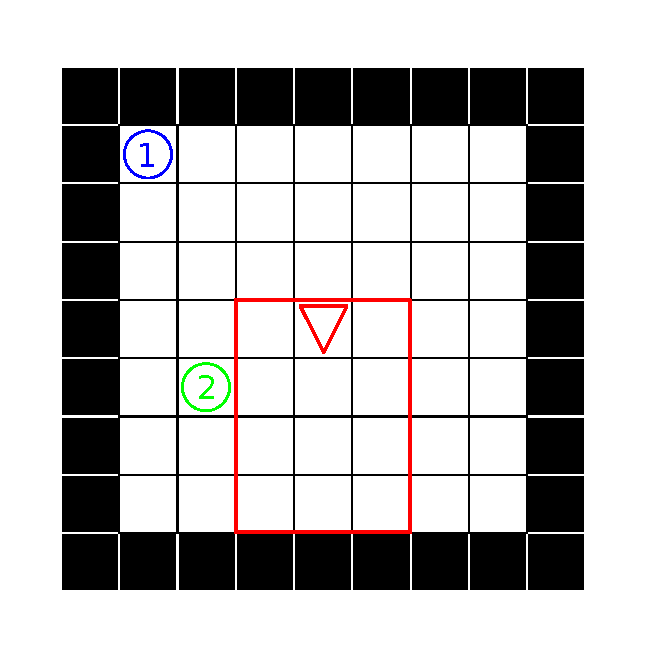
\includegraphics[keepaspectratio,width=\textwidth]{abbildungen/9x9_ep_start.pdf}
    \subcaption{}
    \label{fig_9x9_ep_start}
  \end{subfigure}
  \begin{subfigure}[c]{0.6\textwidth}
    %\centering
    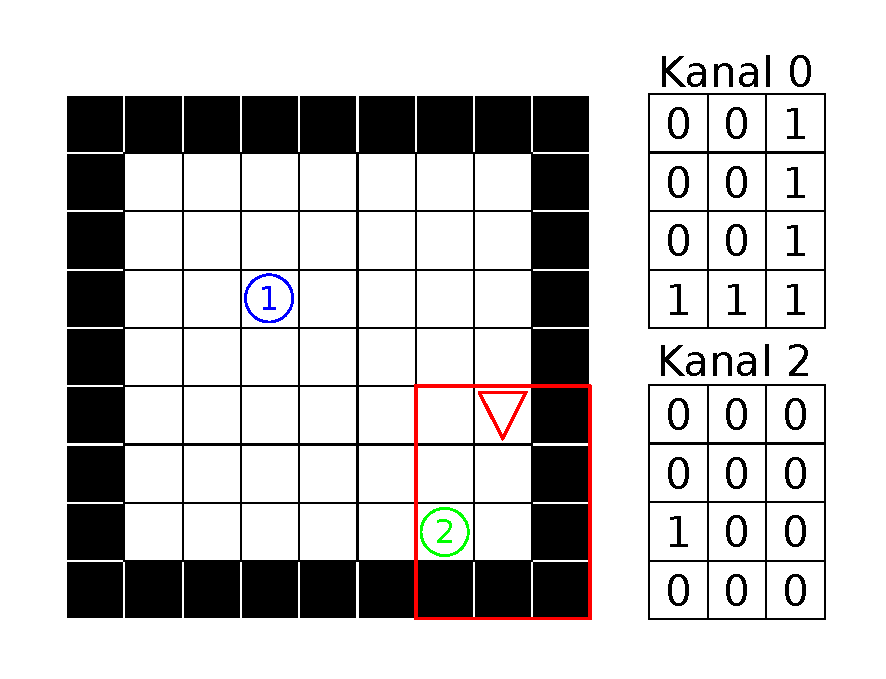
\includegraphics[keepaspectratio,width=\textwidth]{abbildungen/9x9_sample_obs.pdf}
    \subcaption{}
    \label{fig_9x9_sample_obs}
  \end{subfigure}
  \caption{Die linke Abbildung (a) zeigt einen beispielhaften Episodenbeginn. Das rote Dreieck symbolisiert die Startposition und -orientierung des Agenten, das rote Rechteck die Beobachtung und die farbigen Kreise mit den Nummern die entsprechenden Ziele. Die rechte Abbildung (b) verdeutlicht die binäre Kodierung für die Kanäle 0 und 2 anhand einer beispielhaften Beobachtung.}
\end{figure}

Wie zuvor bereits erwähnt ist die Umgebung \glqq One\_Room\_Many\_Goals\_2D\grqq{} eine 2D-Umgebung und besteht aus einem Raum, d.h. einer rechteckigen hindernisfreien Fläche, die von einer durchgehenden Wand umgeben ist. In diesem Raum werden zu Beginn jeder Episode wahlweise zwei, drei oder vier Ziele platziert. Jedes Ziel hat eine eindeutige Nummer zwischen $1$ und $4$. Die Positionen der Ziele werden für jede Episode zufällig neu bestimmt. Dabei gelten folgende Regeln. Zwei aufeinander folgende Ziele dürfen nicht an derselben Position sein, d.h. Ziel 2 darf nicht auf Ziel 1 liegen, Ziel 3 nicht auf Ziel 2 und Ziel 4 nicht auf Ziel 3. Außerdem darf Ziel 1 nicht gleich mit der Startposition des Agenten sein. Der Agent wird zu Beginn jeder Episode auf einer fixen Startposition in der Mitte des Raumes positioniert. Die genauen Koordinaten der Startposition sind von der Größe des Raumes abhängig. Die initiale Blickrichtung des Agenten ist ebenfalls immer gleich, er guckt nach unten. Ein beispielhafter Episodenbeginn, für einen Raum der Größe $9 \times 9$ mit 2 Zielen, ist in Abbildung \ref{fig_9x9_ep_start} dargestellt. Das rote Dreieck markiert die Startposition und -orientierung des Agenten. Das rote Rechteck umfasst die Felder seiner initialen Beobachtung. Die farbigen Kreise mit den Nummern repräsentieren die beiden Ziele. Die Aufgabe des Agenten besteht dann darin, die Ziele in korrekter Reihenfolge abzulaufen, also zuerst Ziel 1, dann Ziel 2, usw. Hierfür erhält er, in Abhängigkeit der Anzahl der Ziele, eine entsprechende Belohnung für jedes Ziel. Dabei ist die Belohnung für das letzte Ziel immer signifikant größer als für die Zwischenziele. Auf diese Weise soll der Agent motiviert werden, alle Ziele zu erreichen. Zum Erledigen der Aufgabe steht dem Agenten eine maximale Anzahl an Schritten zur Verfügung. Diese ist abhängig von der Anzahl der Ziele und der Größe der Umgebung und wird stets so gewählt, dass der Agent nicht jedes Feld der Umgebung so oft ablaufen kann, wie es Ziele gibt. Das Erreichen des Schrittlimits entspricht dem Übergang in einen Terminalzustand. Für diesen Terminalzustand sowie für jeden anderen getätigten Schritt erhält der Agent einen sogenannten Living-Reward von $-1 / Maximale\_Schrittanzahl$. Durch diesen und durch das Schrittlimit soll der Agent dazu animiert werden, die Aufgabe mit möglichst wenigen Schritten zu absolvieren. In Tabelle \ref{belohnung_ormg} ist der Zusammenhang zwischen der Größe der Umgebung, der Anzahl an Zielen, der Belohnungsstruktur und der maximalen Schrittanzahl übersichtlich zusammengefasst.

\begin{table}[h]
  \begin{tabular}{|>{\centering}m{2cm}|>{\centering}m{1.3cm}|>{\centering}m{1.8cm}|>{\centering}m{1.8cm}|>{\centering}m{1.8cm}|>{\centering}m{1.8cm}|>{\centering}m{2.3cm}|} \hline
    Größe der Umgebung & Anzahl Ziele & Belohnung Ziel 1 & Belohnung Ziel 2 & Belohnung Ziel 3 & Belohnung Ziel 4 & Maximale Schrittanzahl \tabularnewline \hline
    9x9 & 2 & 0.2 & 1.0 & - & - & 75 \tabularnewline \hline
    12x12 & 3 & 0.2 & 0.2 & 1.0 & - & 200 \tabularnewline \hline
    15x15 & 4 & 0.2 & 0.2 & 0.2 & 1.0 & 500 \tabularnewline \hline
  \end{tabular}
  \caption{Übersicht über die verschiedenen Größen der Umgebung \glqq One\_Romm\_Many\_Goals\_2D\grqq{} und die daraus resultierende Anzahl an Zielen, Belohnungsstruktur und maximale Schrittanzahl.}
  \label{belohnung_ormg}
\end{table}

Dem Agenten stehen in jedem Schritt drei mögliche Aktionen zur Verfügung: Gehe einen Schritt bzw. Feld nach vorne, also in Blickrichtung, oder drehe dich um $90^\circ$ nach links oder rechts. Dabei kann der Agent nur freie Felder betreten, d.h. wenn der Agent vor sich eine Wand hat und trotzdem einen Schritt nach vorne macht, verändert sich seine Position nicht. Der Zustand $s_t$ ist ein Teilausschnitt der Umgebung in der Größe $(Anzahl\_Ziele + 1) \times 4 \times 3$. Das bedeutet, dass der Agent $4$ Felder geradeaus bzw. in Blickrichtung weit sehen kann. Zur Seite kann er jeweils 1 Feld sehen, sodass sich mit den Feldern links und rechts des Agenten sowie seinem eigenen die $3$ ergibt. Informationen über die Objekte der Umgebung, d.h. die Wände und die Ziele, sind in Analogie zum Neural Map Paper in den $(Anzahl\_Ziele + 1)$ binärkodierten Kanälen enthalten. Dabei enthält der nullte Kanal Informationen über die Lage der Wände. Hierbei entspricht eine $1$ einem Feld mit einer Wand und eine $0$ einem freien Feld. Die Kanäle $1$ bis $4$ spezifizieren die Positionen der entsprechenden Ziele. Dazu enthält der jeweilige Kanal genau eine $1$ an der Position des Ziels, alle anderen Einträge des Kanals sind $0$. In Abbildung \ref{fig_9x9_sample_obs} wird der Zusammenhang zwischem dem Teilauschnitt der Umgebung und dem daraus resultierenden binärkodierten Zustand $s_t$ für die Kanäle 0 und 2 beispielhaft verdeutlicht.

In den folgenden Experimenten werden vier verschiedene Varianten der Neural Map mit einem LSTM als Referenz verglichen. Die erste Variante der Neural Map entspricht der in Abschnitt \ref{sec_nm_impl} beschriebenen Implementierung und kann als eine Grundvariante angesehen werden, da sie soweit möglich den Ausführungen in dem zugrunde liegenden Paper entspricht. Durch die Verwendung der GRU-basierten Local Write Operation entsteht die zweite Variante. Hierbei handelt es sich ebenfalls um eine Grundvariante. Die dritte und vierte Variante entstehen durch die in Abschnitt \ref{sec_write_ext} eingeführte Erweitertung des Schreiboperators, wobei in der vierten Variante zusätzlich die GRU-basierte Schreiboperation verwendet wird. Diese beiden Varianten stellen die im Rahmen dieser Arbeit erdachte Erweiterung der Neural Map dar. Die zum Training verwendeten Hyperparameter des PPO Algorithmus können der Tabelle \ref{hyperparam_ppo_ormg} entnommen werden. Diese sind für alle Experimente basierend auf der Umgebung \glqq One\_Room\_Many\_Goals\_2D\grqq{} und für alle zu untersuchenden Modelle gleich. Lediglich der Parameter $total\_timesteps$, der die für das Training zur Verfügung stehende Gesamtanzahl an Schritten spezifiziert, ist in Abhängigkeit der Umgebungsgröße und der Anzahl an Zielen gewählt worden. Somit wird dieser auch in den entsprechenden Unterabschnitten angegeben. Im Anschluss an das Training werden die Modelle zu Evaluationszwecken für $10^5$ Zeitschritte in der jeweiligen Umgebung ausgeführt.

\begin{table}[h]
  \begin{center}
    \begin{tabular}{1 1}
      \hline
      nsteps & $512$ \\
      ent\_coef & $0,025$ \\
      lr & $3\cdot10^{-4}$ \\
      vf\_coef & $0,5$ \\
      max\_grad\_norm & $0,5$ \\
      gamma & $0,99$ \\
      noptepochs & $1$ \\
      cliprange & $0.2$ \\
      \hline
    \end{tabular}
  \end{center}
  \caption{Übersicht über die zum Training in der Umgebung \glqq One\_Room\_Many\_Goals\_2D\grqq{} verwendeten Hyperparameter des PPO Algorithmus.}
  \label{hyperparam_ppo_ormg}
\end{table}


\subsubsection{Umgebungsgröße 9x9 und 2 Ziele}
Für das erste Experiment werden in einer Umgebung der Größe $9 \times 9$ zwei Ziele platziert. Die Abbildungen \ref{fig_9x9_ep_start} und \ref{fig_9x9_sample_obs} zeigen beispielhaft den Episodenbeginn und einen zufälligen Zeitschritt für die entsprechende Umgebungsgröße und Zielanzahl. Alle Modelle werden zunächst für $2,5\cdot10^6$ Zeitschritte trainiert und anschließend für $10^5$ Zeitschritte zu Evaluationszwecken ausgeführt. Um die Leistungsfähigkeit der verschiedenen Modelle zu vergleichen, werden während der Evaluation sowohl die pro Episode erhaltenen Rewards, als auch die Länge der Episoden aufgezeichnet. Durch die zufällige Platzierung der Ziele variiert auch die Anzahl benötigter Schritte pro Episode und infolgedessen auch der Reward pro Episode. Deshalb wird von diesen beiden Werten jeweils der Durchschnitt aller erfolgreichen Episoden betrachtet. In Tabelle \ref{results9x9} sind die entsprechenden Ergebnisse aller Modelle zusammengefasst. Darüber hinaus enthält sie auch noch die Anzahl erfolgreich absolvierter Episoden. Eine Episode wird als erfolgreich bezeichnet, wenn der Agent innerhalb des Schrittlimits alle Ziele erreicht hat. Hierbei fällt als Erstes auf, dass die Neural Map mit der Erweiterung des Schreiboperators (Neural Map + extW) die besten Ergebnisse erzielt. Sie absolviert in den $10^5$ zur Verfügung stehenden Zeitschritten 4338 erfolgreiche Episoden und benötigt im Durchschnitt für eine erfolgreich absolvierte Episode 21,7 Schritte. Dabei erreicht sie einen durchscnittlichen Reward von 0,91. Die zweitbeste Variante (Neural Map + extW + GRU) benötigt im Durchschnitt 23,7 Schritte, also im Vergleich ungefähr 2 Schritte mehr. Somit erreichen beide Varianten, die die Erweiterung des Schreiboperators verwenden, bessere Ergebnisse als die beiden Grundvarianten. Diese absolvieren eine erfolgreiche Episode im Durchschnitt mit 24,8 (Neural Map) bzw. 25,1 (Neural Map + GRU) Schritten. Die Verwendung der GRU-basierten Local Write Operation bringt hingegen keine Verbesserung und zwar sowohl bezüglich der Grundvariante der Neural Map als auch der Variante mit dem erweiterten Schreiboperator. Abschließend kann noch festgehalten werden, dass alle untersuchten Varianten der Neural Map bessere Ergebnisse erzielen als das LSTM. Dieses benötigt durchschnittlich 26,4 Schritte.

\begin{table}[ht!]
  \begin{tabular}{|>{\centering}m{5cm}|>{\centering}m{2.2cm}|>{\centering}m{3.5cm}|>{\centering}m{3.5cm}|} \hline
    Modell  & Anzahl erfolgreicher Episoden & Durchschnittliche Schrittanzahl pro erfolgreicher Episode & Durchschnittlicher Reward pro erfolgreicher Episode \tabularnewline \hline
    LSTM & 3540 & 26,4 & 0,85 \tabularnewline \hline
    Neural Map & 3854 & 24,8 & 0,87 \tabularnewline \hline
    Neural Map + GRU & 3717 & 25,1 & 0,86 \tabularnewline \hline
    Neural Map + extW & \textbf{4338} & \textbf{21,7} & \textbf{0,91} \tabularnewline \hline
    Neural Map + extW + GRU & 4067 & 23,7 & 0,88 \tabularnewline \hline
  \end{tabular}
  \caption{Übersicht über die Anzahl erfolgreicher Episoden, deren durchschnittliche Länge und durchschnittlicher Reward für die Umgebung \glqq One\_Room\_Many\_Goals\_2D\grqq{} in der Größe $9 \times 9$ mit zwei Zielen.}
  \label{results9x9}
\end{table}

Um einen detailliertern Einblick in das Verhalten der verschiedenen Modelle zu gewinnen, werden während der Evaluation nicht nur der Reward und die Schrittanzahl pro Episode aufgezeichnet, sondern auch die Observationen bzw. Zustände $s_t$, die Rewards $R_t$ und die Positionen des Agenten $(x_t,y_t)$. Hieraus lässt sich für jede Episode der gelaufene Weg des Agenten nachvollziehen. Darüber hinaus können mit diesen Daten die Positionen der Ziele rekonstruiert werden.

Da der Fokus des Experiments darauf liegt, inwiefern der Agent seinen internen Speicher zur Wegfindung nutzen kann, wird im folgenden der Weg vom ersten zum zweiten Ziel detaillierter betrachtet. Dies geschieht aus den folgenden Gründen. Zu Beginn jeder Episode verfügt der Agent logischerweise über keinerlei Wissen bezüglich der Positionen der Ziele. Somit muss er den Raum jedes mal aufs Neue erkunden. Dabei wird er dann irgendwann zufällig auf sein erstes Ziel stoßen. Die dafür benötigte Anzahl von Schritten hängt jedoch in erster Linie von der zufälligen Position des Zieles ab und nicht vom Inhalt bzw. der Nutzung des internen Speichers. Dabei wird angenommen, dass der Agent die Umgebung möglichst effizient erkundet, d.h. bereits gesehene Felder bzw. Bereiche werden nicht mehrfach betreten. Auch wenn der interne Speicher bei einer effizienten Erkundung durchaus von Nutzen sein kann, wird dies wird jedoch vernachlässigt. Somit ist der eigentliche Weg zum ersten Ziel von nachgeordnetem Interesse. Allerdings besteht die Möglichkeit, dass der Agent, während er auf der Suche nach dem ersten Ziel ist, das Zweite bereits sieht. Ist dies der Fall, so ist im Optimalfall der Weg vom ersten zum zweiten Ziel kein rein zufälliger Erkundungsweg mehr, sondern ein zielgerichtetes Wiederauffinden eines zuvor bereits beobachteten Ziels. Um den Weg des Agenten vom ersten zum zweiten Ziel zu bewerten, wird zunächst für jede Episode die optimale Anzahl an Aktionen ermittelt, die für diesen Weg benötigt wird. Diese ergibt sich in erster Linie aus dem Abstand der beiden Ziele, d.h. aus den Beträgen der Differenzen der x- und y-Koordinaten, und den dafür benötigten Schritten. Darüber hinaus werden eventuell noch Drehungen benötigt. In Abhängigkeit der Orientierung des Agenten und der Lage der Ziele ergibt sich die Anzahl benötigter Drehungen entweder zu Null, Eins oder Zwei. Um auf aufwendige Fallunterscheidungen verzichten zu können, wird einfach immer von zwei Drehungen ausgegangen. Somit kann eine pessimistische Schätzung der optimalen Anzahl an Aktionen, um von Ziel i zu Ziel j zu kommen, mit der folgenden Formel berechnet werden:

\begin{equation}
  Optimale\_Schrittanzahl_{i,j} = |x_i - x_j| + |y_i - y_j| + 2
  \label{opt_steps_i_to_j}
\end{equation}

Von diesem Wert wird anschließend der Durchschnitt über alle Episoden gebildet. Ebenso wird für jede Episode die tatsächliche Anzahl benötigter Schritte für den entsprechenden Weg bestimmt, sowie der Durchschnitt über alle Episoden. Diese beiden Durchschnittswerte sowie deren Differenz, die der Anzahl zusätzlicher Schritte entspricht, sind für die betrachteten Modelle in Tabelle \ref{results9x9_1_to_2} zusammengefasst. Es zeigt sich, dass die durchschnittliche optimale Schrittanzahl für alle Modelle sehr ähnlich ist. Die Spannweite ist kleiner als 0,1 Schritte. Somit ist die durchschnittliche Entfernung zwischen den beiden Zielen in den betrachteten Episoden bei allen Modellen sehr ähnlich. Dies verleiht den Werten der tatsächlichen Schrittanzahl bzw. der Anzahl zusätzlicher Schritte mehr Aussagekraft, da diese wiederum immer in Bezug zur optimalen Schrittanzahl betrachtet werden müssen. So macht es einen erheblichen Unterschied, ob der Agent beispielsweise im Durchschnitt 5 zusätzliche Schritte tätigt bezogen auf einen optimalen Weg von 5 oder von 50 Schritten. Die Neural Map mit der Erweiterung des Schreiboperators benötigt die wenigsten zusätzlichen Schritte für den Weg von Ziel 1 zu Ziel 2. Außerdem kommen alle Varianten der Neural Map mit weniger zusätzlichen Schritten aus als das LSTM.

\begin{table}[ht!]
  \begin{tabular}{|>{\centering}m{5cm}|>{\centering}m{2.9cm}|>{\centering}m{2.9cm}|>{\centering}m{3.3cm}|} \hline
    Modell  & Durchschnittliche optimale Schrittanzahl & Durchschnittliche tatsächliche Schrittanzahl & Durchschnittliche Anzahl zusätzlicher Schritte \tabularnewline \hline
    LSTM & 6,7 & 13,7 & 7,0 \tabularnewline \hline
    Neural Map & 6,8 & 13,1 & 6,4 \tabularnewline \hline
    Neural Map + GRU & 6,7 & 13,3 & 6,6 \tabularnewline \hline
    Neural Map + extW & 6,7 & \textbf{12,4} & \textbf{5,7} \tabularnewline \hline
    Neural Map + extW + GRU & 6,7 & 12,9 & 6,2 \tabularnewline \hline
  \end{tabular}
  \caption{Übersicht über die optimale Schrittanzahl, die tatsächliche Schrittanzahl und die Anzahl zusätzlicher Schritte bezogen auf den Weg von Ziel 1 zu Ziel 2 in der Umgebung \glqq One\_Room\_Many\_Goals\_2D\grqq{} in der Größe $9 \times 9$ mit zwei Zielen.}
  \label{results9x9_1_to_2}
\end{table}

Anstatt den Durchschnitt über alle Episoden für den Weg vom ersten zum zweiten Ziel zu betrachten, werden die Episoden im folgenden in drei Mengen aufgeteilt. Alle Episoden, in denen bei der Suche nach dem ersten Ziel das zweite Ziel zu keinem Zeitpunkt gesichtet wurde, bilden die erste Menge. Diese Menge kann in gewisser Weise als Referenz für die beiden anderen Mengen betrachtet werden, da sich bei ihr die zufällige Suche für das zweite Ziel fortsetzt. Die zweite Menge enthält alle Episoden, in denen der Agent mindestens einmal über das zweite Ziel drüber gelaufen ist, d.h. das sich der Agent zu mindestens einem Zeitpunkt an exakt derselben Position wie Ziel 2 befunden hat. Hat der Agent das zweite Ziel lediglich gesichtet, ist jedoch nicht drüber gelaufen, so ist die entsprechende Episode Teil der dritten Menge. Für die drei Mengen werden die Bezeichnungen \glqq Ziel 2 nie beobachtet\grqq{}, \glqq Ziel 2 besucht\grqq{} und \glqq Ziel 2 gesehen\grqq{} verwendet. Auf Basis dieser Mengen soll ergründet werden, ob es einen Unterschied macht beim Wiederauffinden eines Ziels, ob der Agent selbiges in der Vergangenheit nur gesehen hat oder sich bereits an seiner Position befunden hat. Dies ist von Interesse, da der Schreiboperator der Grundvarianten nur die aktuelle Position des Agenten beschreibt, während die Erweiterung auch noch eine zusätzliche Position in Blickrichtung des Agenten beschreibt. Für die Zuordnung der Episoden zu den jeweiligen Mengen werden alle zu einer Episode gehörenden Observationen betrachtet, die auf dem Weg zum ersten Ziel angefallen sind. Von diesen wiederum ist speziell der Teil entscheidend, der mit dem zweiten Kanal bzw. Ziel korrespondiert. Die Unterscheidung zwischen \glqq Ziel\grqq{} besucht und \glqq Ziel\grqq{} gesehen wird vorgenommen, da die Grundvariante der Neural Map nur die Speicherposition beschreibt, die der aktuellen Position des Agenten entspricht. Allerdings enthält die Observation des Agenten nicht nur Informationen über das Feld, auf dem er sich aktuell befindet, sondern auch noch über weitere Felder der Umgebung. Somit soll durch diese Unterscheidung untersucht werden, ob Informationen der Umgebung, die der aktuellen Position des Agenten entsprechen, anders verarbeitet werden beim Beschreiben des internen Speichers, als die restlichen Informationen der Observation. Dazu wird für jede Episode wieder mit der Formel \ref{opt_steps_i_to_j} die optimale Schrittanzahl berechnet. Ebenso wird für jede Episode wieder die tatsächliche Schrittanzahl und die Anzahl zusätzlicher Schritte bestimmt. Auf die Menge \glqq Ziel 2 nie beobachtet\grqq{} entfallen im Durchschnitt über alle Modelle 1452 Episoden, auf die Menge \glqq Ziel 2 besucht\grqq{} 1888 Episoden und auf die Menge \glqq Ziel 2 gesehen\grqq{} 562 Episoden. In Tabelle \ref{results9x9_1_to_2_per_M} sind die Durchschnittswerte der optimalen (Opt) und tatsächlichen Schrittanzahl (Real) für die verschiedenen Mengen für alle Modelle dargestellt. Darüber hinaus ist die zusätzliche Schrittanzahl relativ (rel. Diff) angegeben. Für die relative Differenz fungiert die optimale Schrittanzahl als Bezugsgröße, d.h. die absolute Anzahl zusätzlicher Schritte wird durch diese dividiert und anschließend mit Hundert multipliziert für eine Angabe in Prozent. Die Angabe dieses Wertes soll beim Vergleich der Ergebnisse behilflich sein. Bei den Ergebnissen fällt als Erstes auf, dass die optimale Schrittanzahl zwischen den Zielen für die jeweilige Menge relativ ähnlich ist. So liegt sie für die Menge \glqq Ziel 2 nie beobachtet\grqq{} zwischen 7,5 und 7,6, für die Menge \glqq Ziel 2 besucht\grqq{} zwischen 6,6 und 6,8 und für die Menge \glqq Ziel 2 gesehen\grqq{} zwischen 4,0 und 4,7. Darüber hinaus ist es auffällig, dass in den Episoden der Menge \glqq Ziel 2 gesehen\grqq{} die Ziele 1 und 2 wesentlich näher beieinander liegen als in den anderen beiden Mengen und alle Modelle in dieser Menge die geringste Anzahl zusätzlicher Schritte benötigen. Auch ist die optimale Schrittanzahl für die Menge \glqq Ziel 2 besucht\grqq{} im Durchschnitt um knapp einen Schritt geringer als in der Menge \glqq Ziel 2 nie beobachtet\grqq{}. Bezüglich der beiden Mengen \glqq Ziel 2 nie beobachtet\grqq{} und \glqq Ziel 2 besucht\grqq{} lässt sich bei den verschiedenen Modellen keine Systematik hinsichtlich der Anzahl zusätzlicher Schritte feststellen. Manche Modelle benötigen in der einen Menge weniger zusätzliche Schritte, manche in der Anderen.

\begin{table}
  \begin{tabular}{|c|c|c|c|c|c|c|c|c|c|}
    \hline
    \multirow{3}{*}{Modell} & \multicolumn{3}{|c|}{Ziel 2 nie beobachtet} & \multicolumn{3}{|c|}{Ziel 2 besucht} & \multicolumn{3}{|c|}{Ziel 2 gesehen} \\ \cline{2-10}
    & \multirow{2}{*}{Opt} & \multirow{2}{*}{Real} & rel. & \multirow{2}{*}{Opt} & \multirow{2}{*}{Real} & rel. & \multirow{2}{*}{Opt} & \multirow{2}{*}{Real} & rel. \\
    & & & Diff & & & Diff & & & Diff \\ \hline
    LSTM & 7,5 & 17,1 & 128\% & 6,7 & 13,0 & 94\% & 4,4 & 7,5 & 69\% \\ \hline
    Neural Map & 7,5 & 14,2 & 88\% & 6,8 & 14,1 & 107\% & 4,0 & 5,4 & 36\% \\ \hline
    Neural Map + GRU & 7,6 & 15,2 & 100\% & 6,6 & 13,6 & 105\% & 4,1 & 5,8 & 40\% \\ \hline
    Neural Map + extW & 7,6 & 14,5 & 91\% & 6,8 & 12,7 & 88\% & 4,7 & 7,4 & 57\% \\ \hline
    Neural Map + extW + GRU & 7,6 & 14,8 & 94\% & 6,6 & 13,0 & 96\% & 4,6 & 7,4 & 59\% \\ \hline
  \end{tabular}
  \caption{Übersicht über die optimale (Opt), tatsächliche (Real) und zusätzliche relative Schrittanzahl (rel. Diff) für den Weg von Ziel 1 zu Ziel 2, aufgeteilt in die drei Mengen \glqq Ziel 2 nie beobachtet\grqq{}, \glqq Ziel 2 besucht\grqq{} und \glqq Ziel 2 gesehen\grqq{} für die Umgebung \glqq One\_Room\_Many\_Goals\_2D\grqq{} in der Größe $9 \times 9$ mit zwei Zielen. Die Einteilung in die drei Mengen erfolgt auf Basis der Observationen, die auf dem Weg zu Ziel 1 getätigt werden.}
  \label{results9x9_1_to_2_per_M}
\end{table}


\subsubsection{Umgebungsgröße 12x12 und 3 Ziele}

\begin{figure}[ht!]
  \centering
  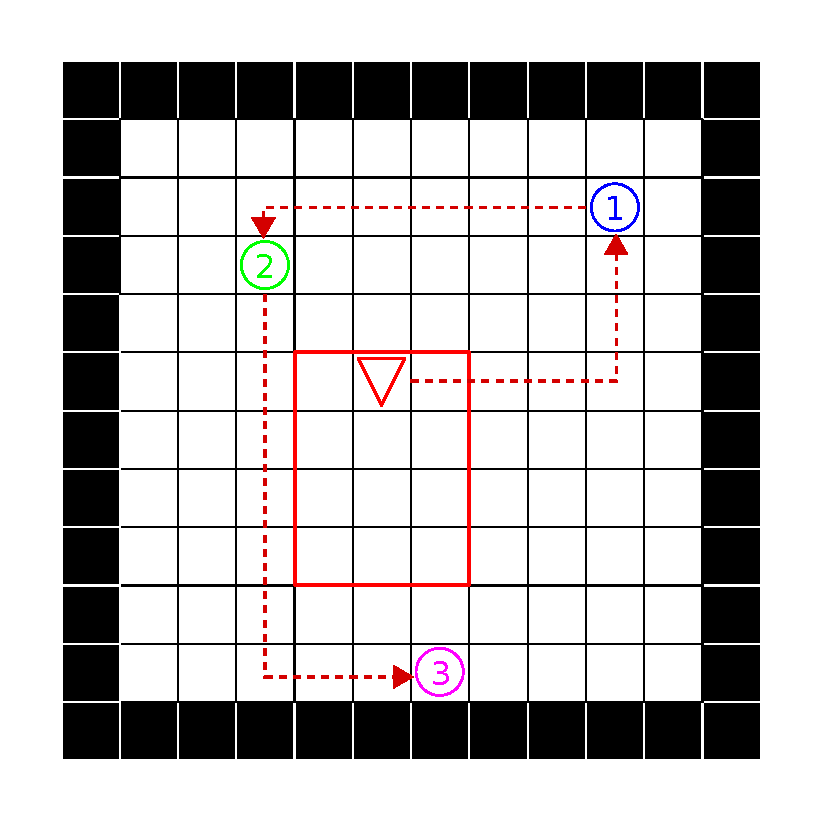
\includegraphics[keepaspectratio,width=0.6\textwidth]{abbildungen/12x12_ep_start.pdf}
  %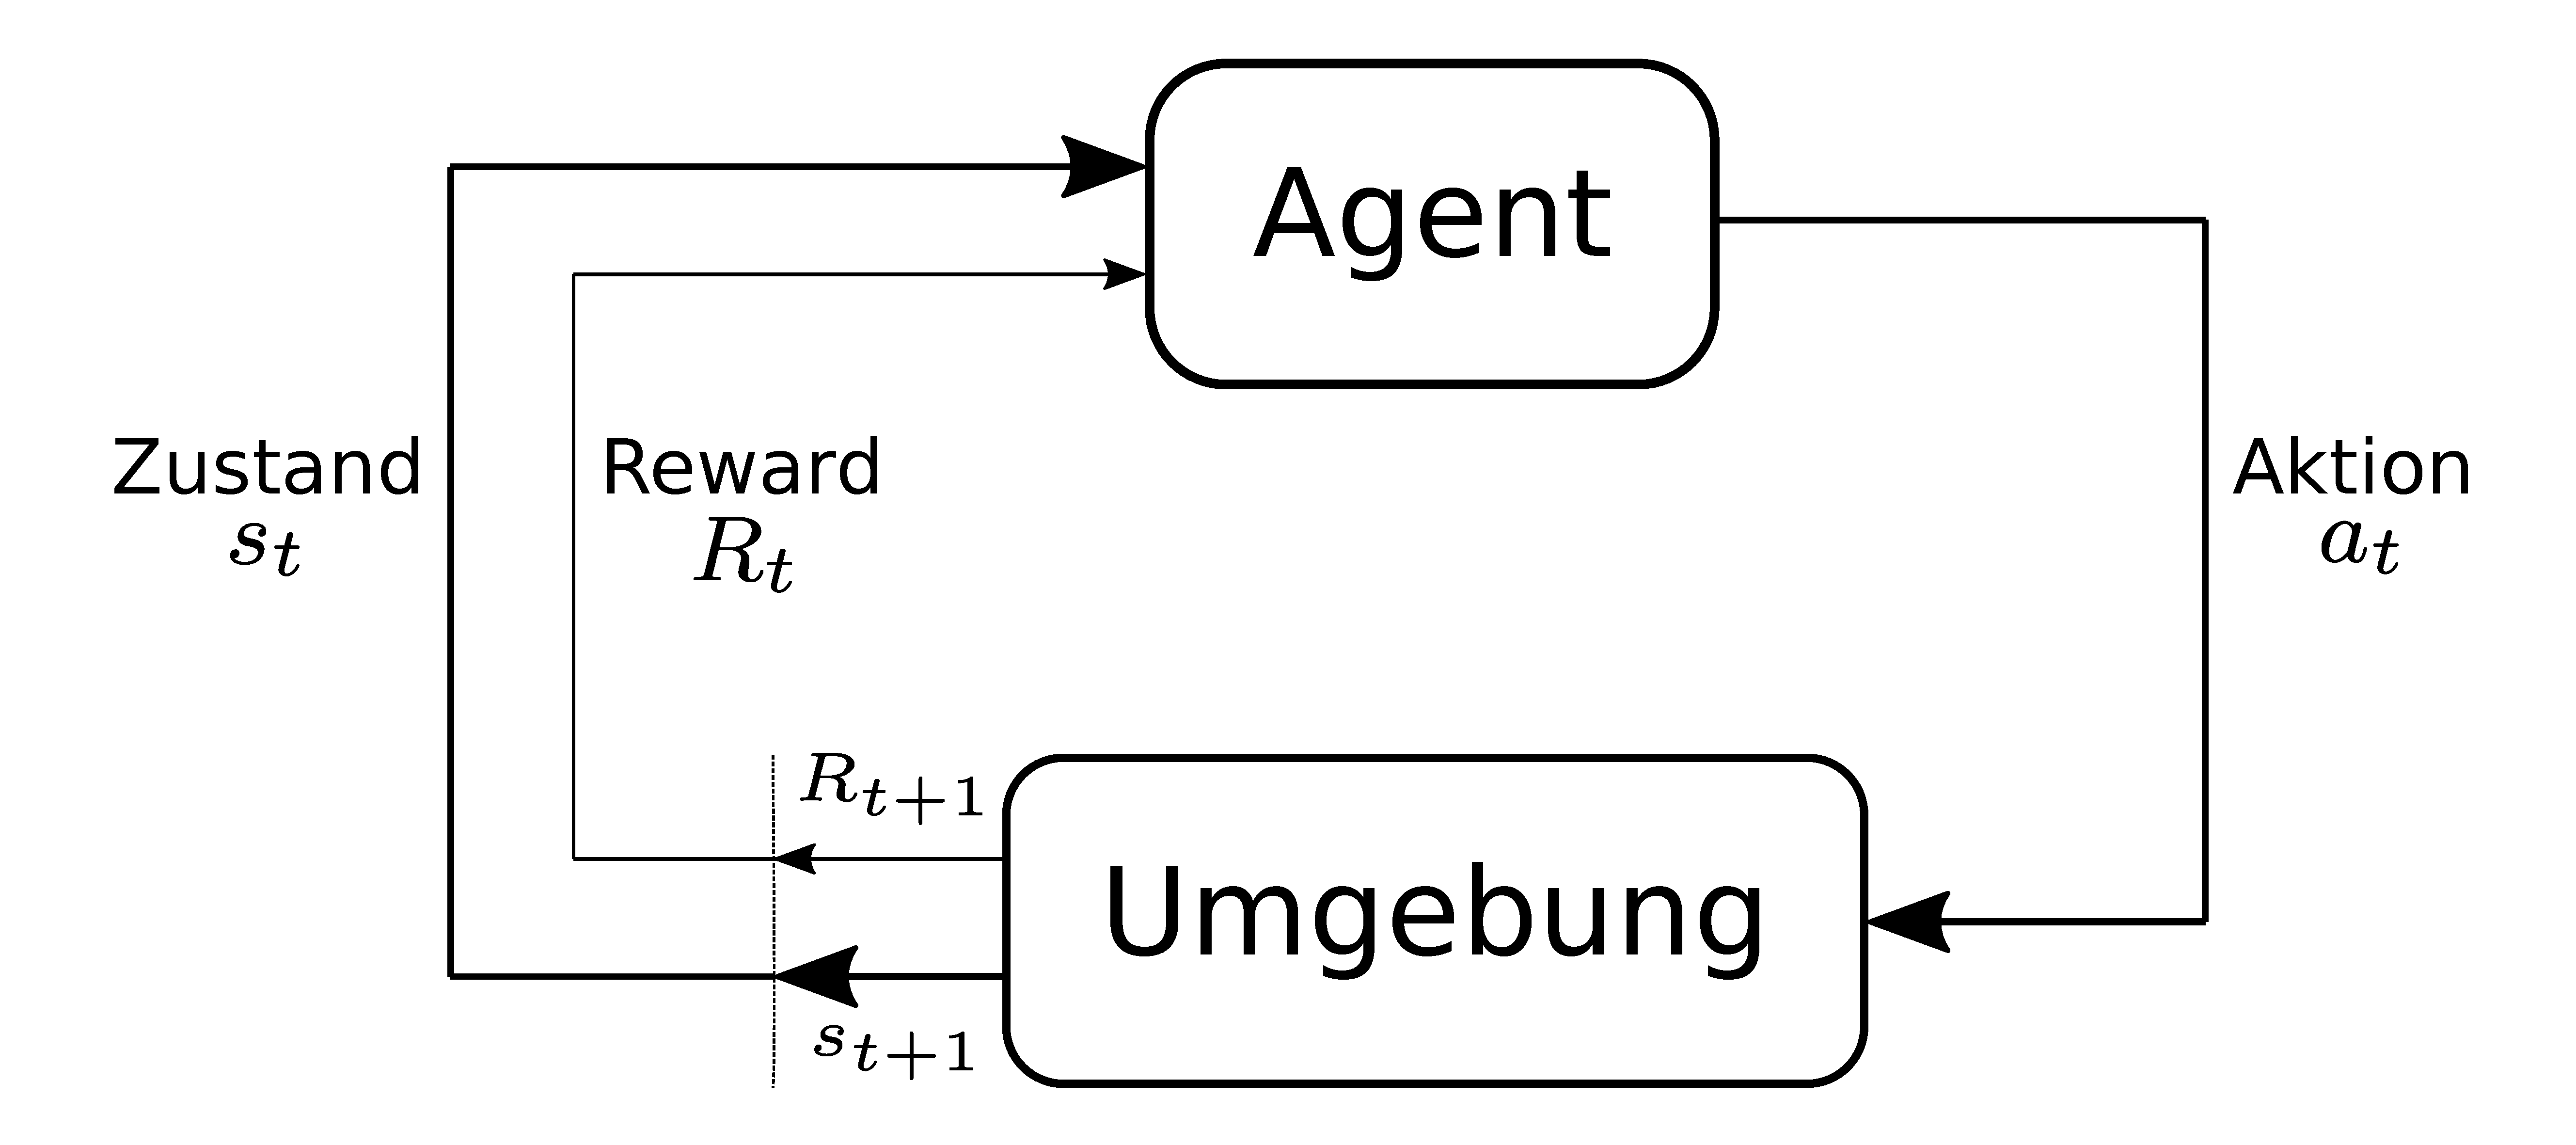
\includegraphics[height=0.5\textwidth, width=0.9\textwidth]{abbildungen/schnittstelle_agent_umgebung.pdf}
  \caption{Die Abbildung zeigt einen beispielhaften Episodenbeginn für die Umgebungsgröße $12 \times 12$ und 3 Ziele. Das rote Dreieck symbolisiert die Startposition und -orientierung des Agenten, das rote Rechteck seine initiale Beobachtung und die farbigen Kreise mit den Nummern die entsprechenden Ziele. Die gestreichelten Pfeile zeigen einen möglichen optimalen Weg.}
  \label{fig_12x12_ep_start}
\end{figure}

Als nächstes wird die Größe der Umgebung auf $12 \times 12$ erhöht und es werden 3 Ziele in ihr platziert. Dadurch wird die Aufgabe für den Agenten anspruchsvoller. Ein beispielhafter Episodenbeginn ist in Abbildung \ref{fig_12x12_ep_start} dargestellt. Neben der Startposition des Agenten, seiner initialen Beobachtung und der Lage der Ziele ist ein möglicher optimaler Weg des Agenten durch die gestrichelten roten Pfeile angedeutet. Das beschreiten dieses Wegs ist jedoch höchst unwahrscheinlich, da der Agent hierfür die Lage der Ziele bereits kennen müsste. Dies ist jedoch selbstverständlich nicht der Fall. Der optimale Weg ist nur zur Veranschaulichung der Problemkomplexität eingezeichnet. In dieser Konfiguration werden alle Modelle für $5\cdot10^6$ Zeitschritte trainiert und anschließend wieder für $10^5$ Zeitschritte evaluiert. Die Auswertung entspricht im Wesentlichen der des vorangegangenen Abschnitts. Zunächst wird die Gesamtleistung der verschiedenen Modelle anhand der Anzahl erfolgreich absolvierter Episoden, der durchschnittlichen Länge und des durchschnittlichen Rewards pro erfolgreicher Episode beurteilt. Die entsprechenden Ergebnisse können der Tabelle \ref{results12x12} entnommen werden. Hierbei erzielen beiden Varianten mit der Erweiterung des Schreiboperators bessere Ergebnisse als die beiden Grundvarianten ohne. Dabei erreicht die Variante der Neural Map mit der Erweiterung des Schreiboperators unter Verwendung des GRU-basierten Schreiboperators das beste Resultat mit durchschnittlich 84,1 Schritten pro erfolgreicher Episode. Die Benutzung der GRU-basierten Schreiboperation verbessert in dieser Konfiguration der Umgebung die jeweilige Neural Map Variante. Des Weiteren liefern alle Varianten der Neural Map wieder bessere Ergebnis als das LSTM.

\begin{table}[ht!]
  \begin{tabular}{|>{\centering}m{5cm}|>{\centering}m{2.2cm}|>{\centering}m{3.5cm}|>{\centering}m{3.5cm}|} \hline
    Modell  & Anzahl erfolgreicher Episoden & Durchschnittliche Schrittanzahl pro erfolgreicher Episode & Durchschnittlicher Reward pro erfolgreicher Episode \tabularnewline \hline
    LSTM & 923 & 92,4 & 0,94 \tabularnewline \hline
    Neural Map & 975 & 88,5 & 0,96 \tabularnewline \hline
    Neural Map + GRU & 983 & 88,1 & 0,96 \tabularnewline \hline
    Neural Map + extW & 995 & 86,7 & 0,97 \tabularnewline \hline
    Neural Map + extW + GRU & \textbf{1053} & \textbf{84,1} & \textbf{0,98} \tabularnewline \hline
  \end{tabular}
  \caption{Übersicht über die Anzahl erfolgreicher Episoden, deren durchschnittliche Länge und durchschnittlicher Reward für die Umgebung \glqq One\_Room\_Many\_Goals\_2D\grqq{} in der Größe $12 \times 12$ mit drei Zielen.}
  \label{results12x12}
\end{table}

Mit der gleichen Begründung, wie im vorherigen Abschnitt, wird als nächstes wieder der Weg vom ersten zum zweiten Ziel detailierter untersucht. Dabei werden die Episoden wieder in die drei zuvor definierten Mengen aufgeteilt. Hierbei ergibt sich, dass die Menge \glqq Ziel 2 nie beobachtet\grqq{} im Durchschnitt über alle Modelle 411 Episoden besitzt, die Menge \glqq Ziel 2 besucht\grqq{} 477 Episoden und die Menge \glqq Ziel 2 gesehen\grqq{} 86 Episoden. Für jede Menge wird wieder die durchschnittliche optimale, tatsächliche und relative zusätzliche Schrittanzahl berechnet. Die entsprechenden Ergebnisse können der Tabelle \ref{results12x12_1_to_2_per_M} entnommen werden. Es fällt auf, dass der durchschnittliche optimale Weg für die Menge \glqq Ziel 2 gesehen\grqq{} erheblich geringer ist, als für die beiden anderen Mengen. Darüber hinaus benötigen alle Varianten der Neural Map in dieser Menge relativ betrachtet die geringste Anzahl zusätzlicher Schritte. Weiterhin kann beobachtet werden, dass die optimale Schrittanzahl für die Menge \glqq Ziel 2 nie beobachtet\grqq{} geringfügig größer ist als für die Menge \glqq Ziel 2 besucht\grqq{}. Hinsichtlich der zusätzlichen Schrittanzahl lässt sich, bezüglich dieser beiden Mengen, wieder keine eindeutige Systematik feststellen. Manche Modelle benötigen in der einen Menge weniger zusätzliche Schritte, manche in der anderen. Wobei die Unterschiede teilweise auch sehr gering sind, z.B 261\% zu 257\% für die Variante Neural Map + extW + GRU.

\begin{table}
  \begin{tabular}{|c|c|c|c|c|c|c|c|c|c|}
    \hline
    \multirow{3}{*}{Modell} & \multicolumn{3}{|c|}{Ziel 2 nie beobachtet} & \multicolumn{3}{|c|}{Ziel 2 besucht} & \multicolumn{3}{|c|}{Ziel 2 gesehen} \\ \cline{2-10}
    & \multirow{2}{*}{Opt} & \multirow{2}{*}{Real} & rel. & \multirow{2}{*}{Opt} & \multirow{2}{*}{Real} & rel. & \multirow{2}{*}{Opt} & \multirow{2}{*}{Real} & rel. \\
    & & & Diff & & & Diff & & & Diff \\ \hline
    LSTM & 9,2 & 32,5 & 254\% & 8,6 & 31,7 & 270\% & 4,4 & 16,0 & 264\% \\ \hline
    Neural Map & 8,4 & 34,4 & 312\% & 7,8 & 29,7 & 279\% & 4,1 & 9,7 & 138\% \\ \hline
    Neural Map + GRU & 8,7 & 32,0 & 279\% & 8,3 & 30,5 & 268\% & 3,7 & 11,1 & 202\% \\ \hline
    Neural Map + extW & 9,1 & 32,0 & 253\% & 8,2 & 30,9 & 277\% & 3,9 & 9,5 & 141\% \\ \hline
    Neural Map + extW + GRU & 9,1 & 33,0 & 261\% & 8,4 & 29,9 & 257\% & 4,5 & 13,8 & 208\% \\ \hline
  \end{tabular}
  \caption{Übersicht über die optimale (Opt), tatsächliche (Real) und zusätzliche relative Schrittanzahl (rel. Diff) für den Weg von Ziel 1 zu Ziel 2, aufgeteilt in die drei Mengen \glqq Ziel 2 nie beobachtet\grqq{}, \glqq Ziel 2 besucht\grqq{} und \glqq Ziel 2 gesehen\grqq{} für die Umgebung \glqq One\_Room\_Many\_Goals\_2D\grqq{} in der Größe $12 \times 12$ mit drei Zielen. Die Einteilung in die drei Mengen erfolgt auf Basis der Observationen, die auf dem Weg zu Ziel 1 getätigt werden.}
  \label{results12x12_1_to_2_per_M}
\end{table}

Durch die Verwendung von 3 Zielen bietet sich die Möglichkeit, neben dem Weg von Ziel 1 zu Ziel 2, auch noch den Weg von Ziel 2 zu Ziel 3 detaillierter zu betrachten. Das Interesse an einer entsprechenden Untersuchung dieses Wegs lässt sich ähnlich begründen, wie für den Weg von Ziel 1 zu Ziel 2. Darüber hinaus findet die Aufteilung der Episoden in die drei Mengen \glqq Ziel 3 nie beobachtet\grqq{}, \glqq Ziel 3 besucht\grqq{} und \glqq Ziel 3 gesehen\grqq{} auf Basis der Observationen statt, die auf dem gesamten Weg zu Ziel 2 anfallen. Dieser ist logischerweise länger als der Weg zu Ziel 1, der wiederum für die Mengeneinteilung in der Analyse des Weges von Ziel 1 zu Ziel 2 verantwortlich war. Aufgrund des längeren Weges zu Ziel 2 kann angenommen werden, dass der Agent die Umgebung umfangreicher erkundet hat. Ob sich dies auch in den Ergebnissen für den Weg von Ziel 2 zu Ziel 3 niederschlägt, soll im Weiteren versucht werden zu beantworten. Zuerst ergibt sich folgende Einteilung der Mengen. Dabei enthält die Menge \glqq Ziel 3 nie beobachtet\grqq{} im Durchschnitt über alle Modelle 182 Episoden, die Menge \glqq Ziel 3 besucht\grqq{} 754 Episoden und die Menge \glqq Ziel 3 gesehen\grqq{} 38 Episoden. Bei den in Tabelle \ref{results12x12_2_to_3_per_M} dargestellten Ergebnissen fällt zunächst wieder auf, dass der optimale Weg für die Menge \glqq Ziel 3 gesehen\grqq{} wieder erheblich geringer ist, als für die beiden anderen Mengen. Jedoch erzielen dieses Mal nicht alle Modelle in dieser Menge die geringste Anzahl zusätzlicher Schritte. Dies ist lediglich der Fall für die beiden Varianten der Neural Map, die die GRU-basierte Schreiboperation verwenden. Des Weiteren ist der optimale Weg für die Menge \glqq Ziel 3 nie beobachtet\grqq{} um gut einen Schritt größer als für die Menge \glqq Ziel 3 besucht\grqq{}. Bis auf die Grundvariante der Neural Map benötigen alle anderen Modelle in der Menge \glqq Ziel 3 besucht\grqq{} weniger zusätzliche Schritte. Insbesondere für die beiden Varianten, die die GRU-basierte Schreiboperation benutzen, fällt der Unterschied sehr deutlich aus.


\begin{table}
  \begin{tabular}{|c|c|c|c|c|c|c|c|c|c|}
    \hline
    \multirow{3}{*}{Modell} & \multicolumn{3}{|c|}{Ziel 3 nie beobachtet} & \multicolumn{3}{|c|}{Ziel 3 besucht} & \multicolumn{3}{|c|}{Ziel 3 gesehen} \\ \cline{2-10}
    & \multirow{2}{*}{Opt} & \multirow{2}{*}{Real} & rel. & \multirow{2}{*}{Opt} & \multirow{2}{*}{Real} & rel. & \multirow{2}{*}{Opt} & \multirow{2}{*}{Real} & rel. \\
    & & & Diff & & & Diff & & & Diff \\ \hline
    LSTM & 9,7 & 36,7 & 276\% & 8,7 & 30,3 & 249\% & 5,2 & 19,5 & 277\% \\ \hline
    Neural Map & 10,0 & 35,0 & 250\% & 8,2 & 29,9 & 264\% & 4,7 & 19,5 & 314\% \\ \hline
    Neural Map + GRU & 9,8 & 39,4 & 301\% & 8,6 & 29,0 & 236\% & 5,9 & 14,5 & 148\% \\ \hline
    Neural Map + extW & 9,6 & 33,9 & 253\% & 8,4 & 28,8 & 244\% & 5,5 & 19,6 & 256\% \\ \hline
    Neural Map + extW + GRU & 9,9 & 35,3 & 258\% & 8,3 & 25,6 & 207\% & 4,4 & 10,1 & 130\% \\ \hline
  \end{tabular}
  \caption{Übersicht über die optimale (Opt), tatsächliche (Real) und zusätzliche relative Schrittanzahl (rel. Diff) für den Weg von Ziel 2 zu Ziel 3, aufgeteilt in die drei Mengen \glqq Ziel 3 nie beobachtet\grqq{}, \glqq Ziel 3 besucht\grqq{} und \glqq Ziel 3 gesehen\grqq{} für die Umgebung \glqq One\_Room\_Many\_Goals\_2D\grqq{} in der Größe $12 \times 12$ mit drei Zielen. Die Einteilung in die drei Mengen erfolgt auf Basis der Observationen, die auf dem Weg zu Ziel 2 getätigt werden.}
  \label{results12x12_2_to_3_per_M}
\end{table}



\subsubsection{Umgebungsgröße 15x15 und 4 Ziele}

\begin{figure}[ht!]
  \centering
  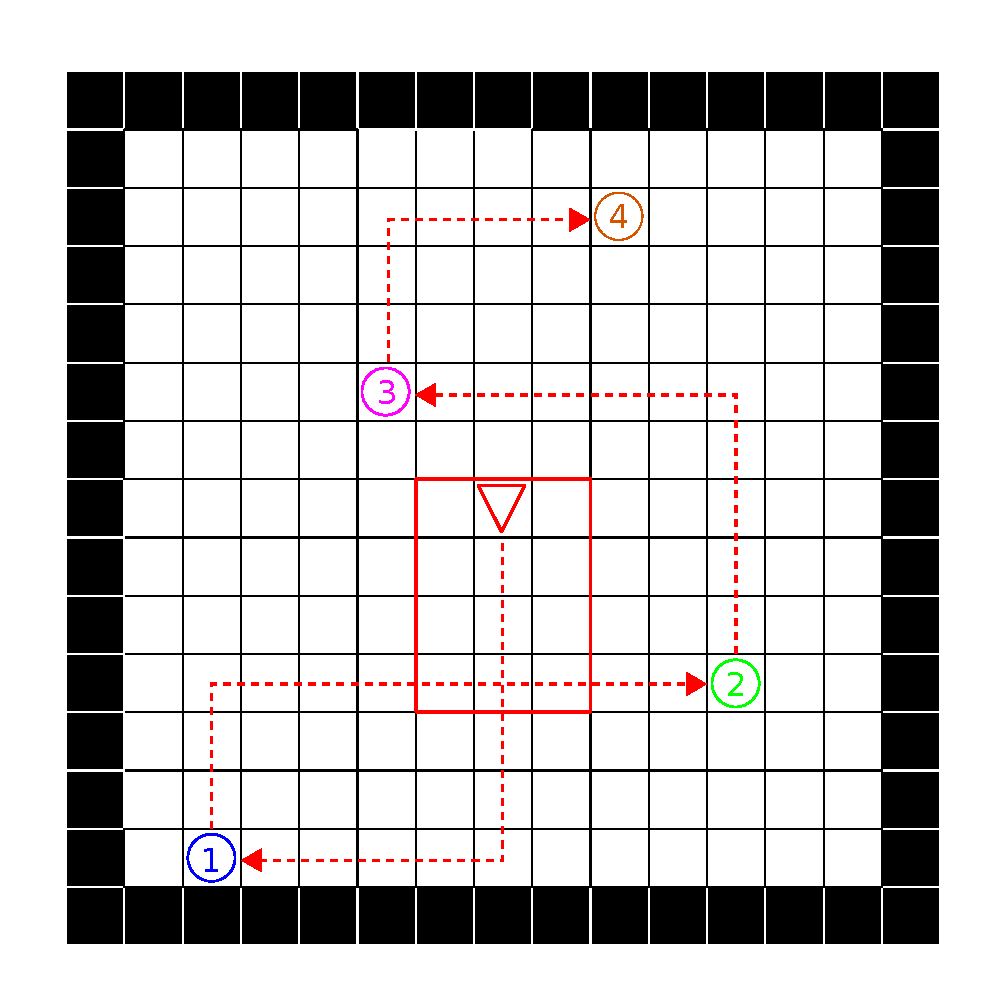
\includegraphics[keepaspectratio,width=0.65\textwidth]{abbildungen/15x15_ep_start.pdf}
  %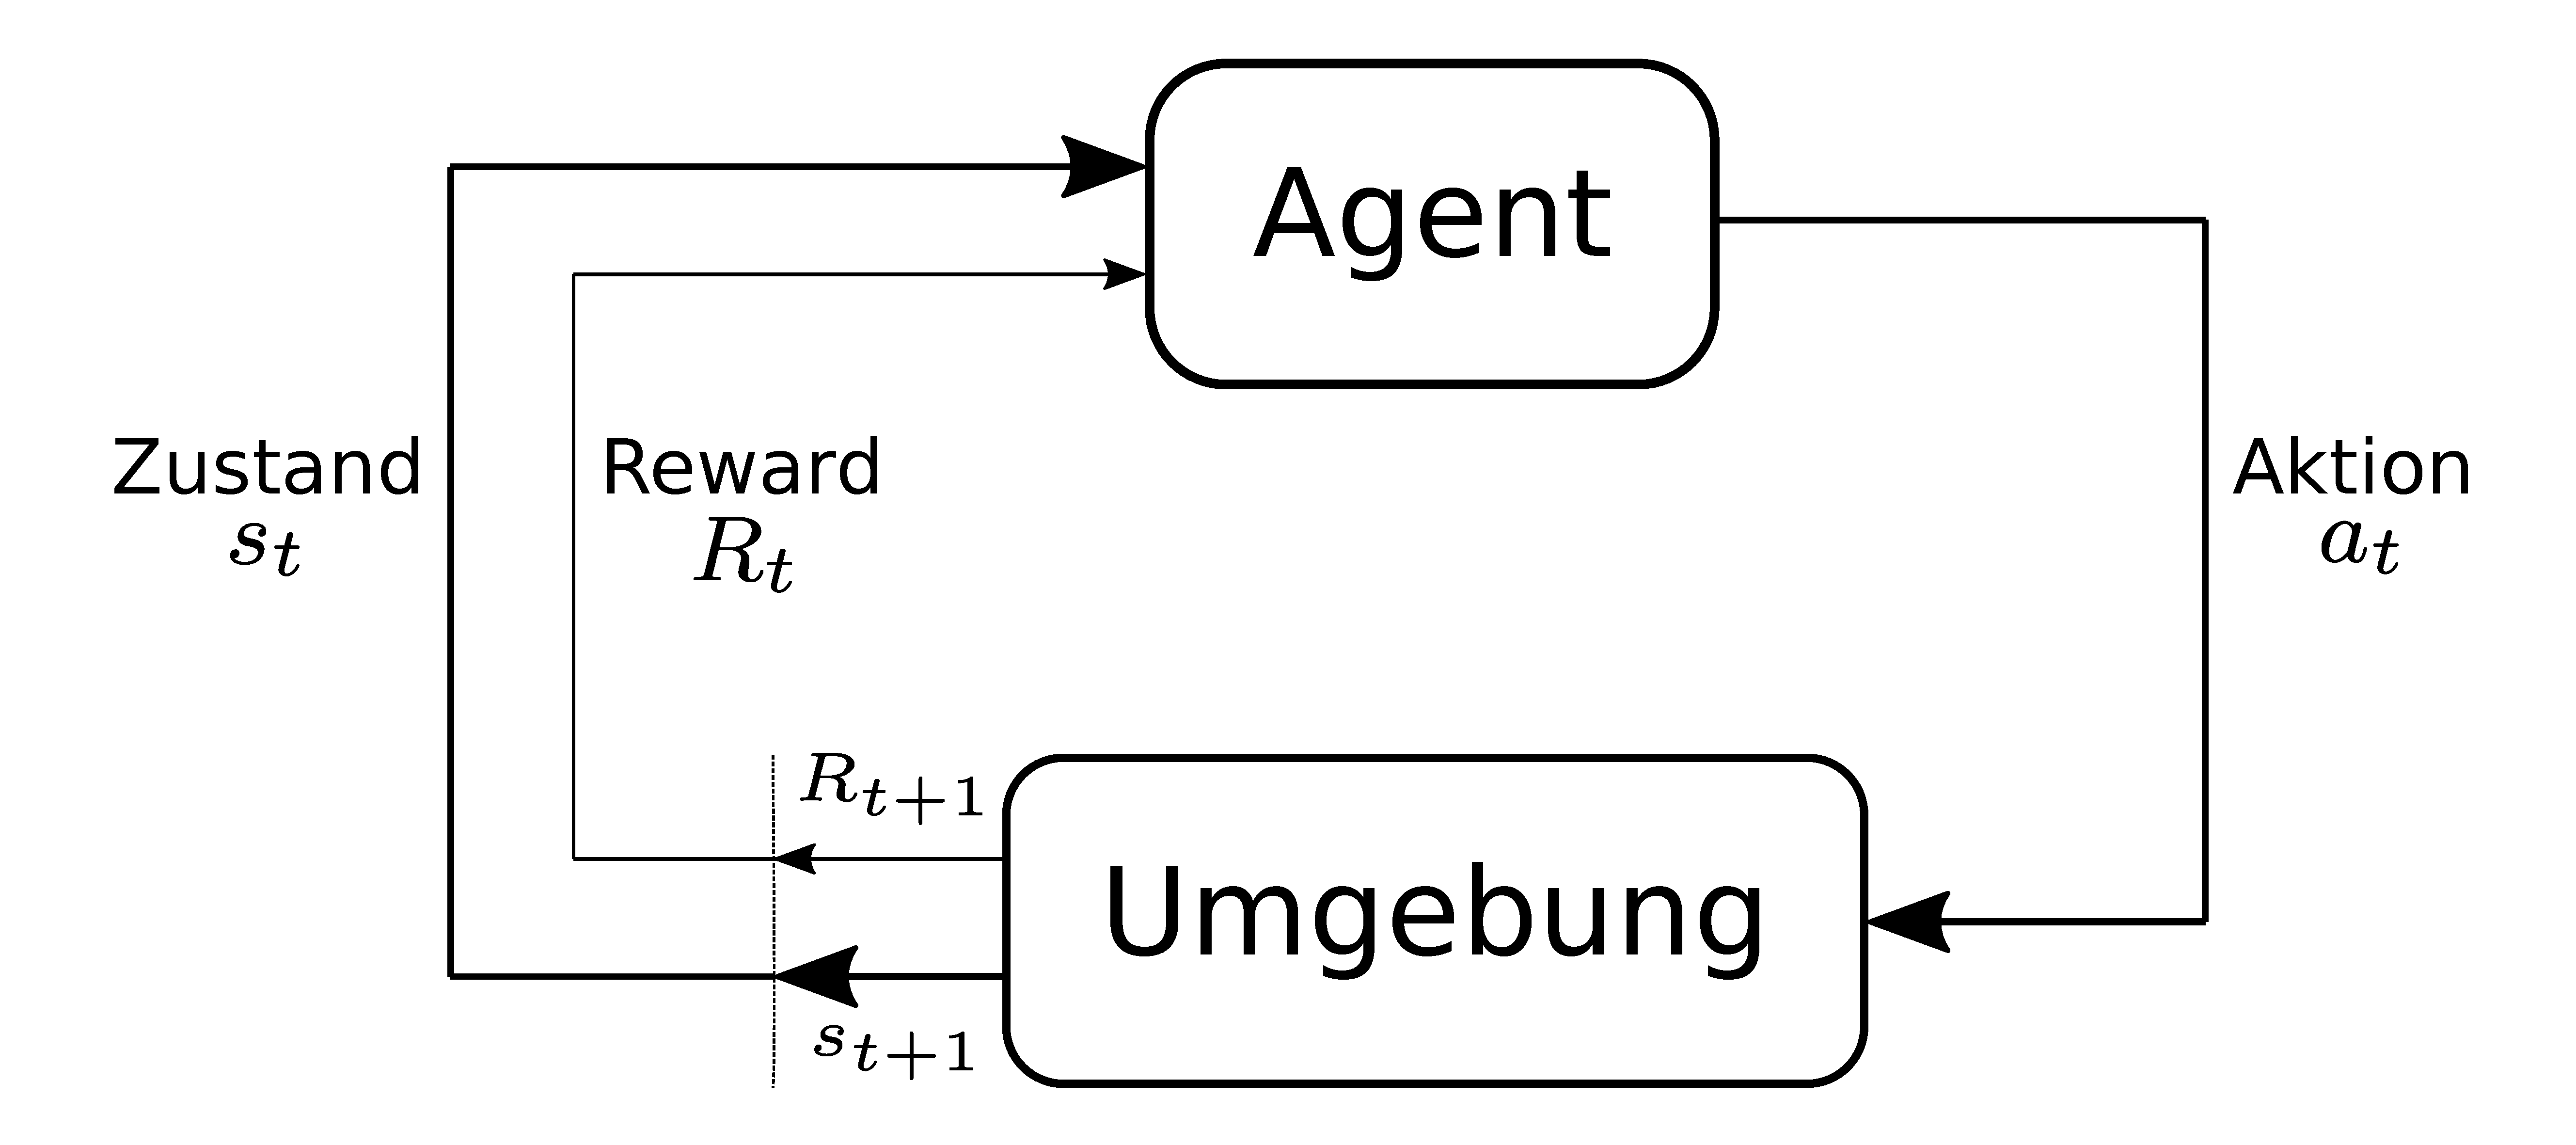
\includegraphics[height=0.5\textwidth, width=0.9\textwidth]{abbildungen/schnittstelle_agent_umgebung.pdf}
  \caption{Die Abbildung zeigt einen beispielhaften Episodenbeginn für die Umgebungsgröße $15 \times 15$ und 4 Ziele. Das rote Dreieck symbolisiert Startposition und -orientierung des Agenten, das rote Rechteck seine initiale Beobachtung und die farbigen Kreise mit den Nummern die entsprechenden Ziele. Die gestrichelten Pfeile zeigen einen möglichen optimalen Weg.}
  \label{fig_15x15_ep_start}
\end{figure}

Zum Abschluss der Experimente, basierend auf der Umgebung \glqq One\_Room\_Many\_Goals\grqq{}, wird die Umgebungsgröße als $15 \times 15$ gewählt und es werden 4 Ziele platziert. Auf diese Weise wird die Schwierigkeit der Aufgabe ein weiteres Mal erhöht. Die Abbildung \ref{fig_15x15_ep_start} zeigt einen beispielhaften Episodenbeginn. Die gestrichelten roten Pfeile symbolisieren erneut einen möglichen optimalen Weg und sollen die gesteigerte Problemkomplexität verdeutlichen. In dieser Konfiguration werden alle Modelle für $10\cdot10^6$ Zeitschritte trainiert, ehe sie wieder für $10^5$ Schritte evaluiert werden. Die Auswertung folgt dem Vorgehen der beiden vorangegangenen Abschnitte. Folglich können der Tabelle \ref{results15x15} die Anzahl erfolgreicher Episoden und die durchschnittliche Schritttanzahl, sowie der durchschnittliche Reward für selbige entnommen werden. Die besten Resultate erzielt die Neural Map mit der Erweiterung des Schreiboperators unter Verwendung der GRU-basierten Schreiboperation (Neural Map + extW + GRU). Sie absolviert 404 erfolgreiche Episoden, benötigt dafür im Schnitt 224,7 Schritte und erzielt einen durchschnittlichen Reward von 1,15. Gefolgt wird sie von der Variante mit der Erweiterung des Schreiboperators (Neural Map + extW). Somit erreichen beide Varianten mit der Erweiterung des Schreiboperators bessere Ergebnisse als die Grundvarianten. Darüber hinaus verbessert die Verwendung der GRU-basierten Schreiboperation die jeweilige Variante. Ebenso liefern alle Varianten der Neural Map wieder bessere Resultate als das LSTM.

\begin{table}[ht!]
  \begin{tabular}{|>{\centering}m{5cm}|>{\centering}m{2.2cm}|>{\centering}m{3.5cm}|>{\centering}m{3.5cm}|} \hline
    Modell  & Anzahl erfolgreicher Episoden & Durchschnittliche Schrittanzahl pro erfolgreicher Episode & Durchschnittlicher Reward pro erfolgreicher Episode \tabularnewline \hline
    LSTM & 329 & 269,8 & 1,08 \tabularnewline \hline
    Neural Map & 365 & 242,1 & 1,12 \tabularnewline \hline
    Neural Map + GRU & 360 & 239,4 & 1,12 \tabularnewline \hline
    Neural Map + extW & 397 & 230,3 & 1,14 \tabularnewline \hline
    Neural Map + extW + GRU & \textbf{404} & \textbf{224,7} & \textbf{1,15} \tabularnewline \hline
  \end{tabular}
  \caption{Übersicht über die Anzahl erfolgreicher Episoden, deren durchschnittliche Länge und durchschnittlicher Reward für die Umgebung \glqq One\_Room\_Many\_Goals\_2D\grqq{} in der Größe $15 \times 15$ mit vier Zielen.}
  \label{results15x15}
\end{table}

Im Folgenden wird wie zuvor auch der Weg von Ziel 1 zu Ziel 2 wieder genauer untersucht. Das Vorgehen ist dabei analog zu den beiden vorherigen Experimenten. Somit werden die Episoden zunächst wieder in die entsprechenden Mengen unterteilt, wobei die Menge \glqq Ziel 2 nie beobachtet\grqq{} durchschnittlich über 162 Episoden verfügt, die Menge \glqq Ziel 2 besucht\grqq{} über 189 Episoden und die Menge \glqq Ziel 2 gesehen\grqq{} über 25 Episoden. Die entsprechenden Ergebnisse befinden sich in Tabelle \ref{results15x15_1_to_2_per_M}. Erneut fällt als Erstes auf, dass der optimale Weg für die Menge \glqq Ziel 2 gesehen\grqq{} erheblich kleiner ist, als für die beiden anderen Mengen. Darüber hinaus ist der optimale Weg für die Menge \glqq Ziel 2 nie beobachtet\grqq{} wieder ungefähr einen Schritt länger als für die Menge \glqq Ziel 2 besucht \grqq{}. Dieses Mal benötigen alle Modelle in der Menge \glqq Ziel 2 besucht\grqq{} weniger zusätzliche Schritte als in der Menge \glqq Ziel 2 nie beobachtet\grqq{}, wobei der Unterschied für die Grundvariante der Neural Map am größten ist mit 504\% im Vergleich zu 644\%. Außerdem benötigen alle Modelle bis auf die Variante mit der Erweiterung des Schreiboperators (Neural Map + extW) in der Menge \glqq Ziel 2 beobachtet\grqq{} die geringste Anzahl zusätzlicher Schritte.

\begin{table}
  \begin{tabular}{|c|c|c|c|c|c|c|c|c|c|}
    \hline
    \multirow{3}{*}{Modell} & \multicolumn{3}{|c|}{Ziel 2 nie beobachtet} & \multicolumn{3}{|c|}{Ziel 2 besucht} & \multicolumn{3}{|c|}{Ziel 2 gesehen} \\ \cline{2-10}
    & \multirow{2}{*}{Opt} & \multirow{2}{*}{Real} & rel. & \multirow{2}{*}{Opt} & \multirow{2}{*}{Real} & rel. & \multirow{2}{*}{Opt} & \multirow{2}{*}{Real} & rel. \\
    & & & Diff & & & Diff & & & Diff \\ \hline
    LSTM & 11,5 & 80,4 & 598\% & 10,5 & 63,7 & 505\% & 5,3 & 36,6 & 586\% \\ \hline
    Neural Map & 10,6 & 78,9 & 644\% & 10,3 & 62,0 & 504\% & 5,8 & 51,5 & 784\% \\ \hline
    Neural Map + GRU & 11,3 & 67,4 & 498\% & 10,3 & 59,8 & 481\% & 4,5 & 31,7 & 598\% \\ \hline
    Neural Map + extW & 11,4 & 64,0 & 461\% & 10,1 & 55,3 & 447\% & 6,0 & 30,8 & 413\% \\ \hline
    Neural Map + extW + GRU & 11,0 & 60,9 & 453\% & 10,6 & 54,4 & 415\% & 5,3 & 28,0 & 427\% \\ \hline
  \end{tabular}
  \caption{Übersicht über die optimale (Opt), tatsächliche (Real) und zusätzliche relative Schrittanzahl (rel. Diff) für den Weg von Ziel 1 zu Ziel 2 aufgeteilt in die drei Mengen \glqq Ziel 2 nie beobachtet\grqq{}, \glqq Ziel 2 besucht\grqq{} und \glqq Ziel 2 gesehen\grqq{} für die Umgebung \glqq One\_Room\_Many\_Goals\_2D\grqq{} in der Größe $15 \times 15$ mit vier Zielen. Die Einteilung in die drei Mengen erfolgt auf Basis der Observationen, die auf dem Weg zu Ziel 1 getätigt werden.}
  \label{results15x15_1_to_2_per_M}
\end{table}

Der Weg von Ziel 2 zu Ziel 3 wird ebenfalls wieder im Detail analysiert. Hierbei hat die Menge \glqq Ziel 3 nie beobachtet\grqq{} durchschnittlich 74 Episoden, die Menge \glqq Ziel 3 besucht\grqq{} 288 Episoden und die Menge \glqq Ziel 3 gesehen\grqq{} 14 Episoden. Die dazugehörigen Ergebnisse sind in der Tabelle \ref{results15x15_2_to_3_per_M} abgebildet. Erneut ist der optimale Weg für die Menge \glqq Ziel 3 gesehen\grqq{} im Durchschnitt wesentlich kürzer als für die beiden anderen Mengen. Ebenso ist der optimale Weg für die Menge \glqq Ziel 3 nie beobacht\grqq{} wieder ungefähr um einen Schritt größer als für die Menge \glqq Ziel 3 besucht\grqq{}. Darüber hinaus kann keine Systematik beobacht werden, wenn es darum geht, in welcher Menge die Modelle die geringste Anzahl zusätzlicher Schritte tätigen.

\begin{table}
  \begin{tabular}{|c|c|c|c|c|c|c|c|c|c|}
    \hline
    \multirow{3}{*}{Modell} & \multicolumn{3}{|c|}{Ziel 3 nie beobachtet} & \multicolumn{3}{|c|}{Ziel 3 besucht} & \multicolumn{3}{|c|}{Ziel 3 gesehen} \\ \cline{2-10}
    & \multirow{2}{*}{Opt} & \multirow{2}{*}{Real} & rel. & \multirow{2}{*}{Opt} & \multirow{2}{*}{Real} & rel. & \multirow{2}{*}{Opt} & \multirow{2}{*}{Real} & rel. \\
    & & & Diff & & & Diff & & & Diff \\ \hline
    LSTM & 11,0 & 70,3 & 538\% & 10,5 & 61,1 & 484\% & 4,8 & 23,3 & 391\% \\ \hline
    Neural Map & 11,3 & 66,8 & 490\% & 10,3 & 59,6 & 481\% & 7,1 & 55,6 & 687\% \\ \hline
    Neural Map + GRU & 11,6 & 65,8 & 466\% & 10,0 & 60,3 & 504\% & 5,0 & 31,4 & 527\% \\ \hline
    Neural Map + extW & 10,7 & 63,3 & 489\% & 10,1 & 59,9 & 493\% & 6,5 & 46,3 & 609\% \\ \hline
    Neural Map + extW + GRU & 11,6 & 67,3 & 482\% & 10,6 & 59,0 & 454\% & 5,3 & 17,6 & 231\% \\ \hline
  \end{tabular}
  \caption{Übersicht über die optimale (Opt), tatsächliche (Real) und zusätzliche relative Schrittanzahl (rel. Diff) für den Weg von Ziel 2 zu Ziel 3 aufgeteilt in die drei Mengen \glqq Ziel 3 nie beobachtet\grqq{}, \glqq Ziel 3 besucht\grqq{} und \glqq Ziel 3 gesehen\grqq{} für die Umgebung \glqq One\_Room\_Many\_Goals\_2D\grqq{} in der Größe $15 \times 15$ mit vier Zielen. Die Einteilung in die drei Mengen erfolgt auf Basis der Observationen, die auf dem Weg zu Ziel 2 getätigt werden.}
  \label{results15x15_2_to_3_per_M}
\end{table}


\iffalse
\begin{table}
  \begin{tabular}{|c|c|c|c|c|c|c|c|c|c|}
    \hline
    \multirow{3}{*}{Modell} & \multicolumn{3}{|c|}{Ziel 4 nie beobachtet} & \multicolumn{3}{|c|}{Ziel 4 besucht} & \multicolumn{3}{|c|}{Ziel 4 gesehen} \\ \cline{2-10}
    & \multirow{2}{*}{Opt} & \multicolumn{2}{|c|}{Differenz} & \multirow{2}{*}{Opt} & \multicolumn{2}{|c|}{Differenz} & \multirow{2}{*}{Opt} & \multicolumn{2}{|c|}{Differenz} \\ \cline{3-4} \cline{6-7} \cline{9-10}
    & & abs. & rel. & & abs. & rel. & & abs. & rel. \\ \hline
    LSTM & 12,47 & 72,17 & 578\% & 10,89 & 50,16 & 461\% & 6,4 & 36,6 & 572\% \\ \hline
    Neural Map & 12,17 & 41,79 & 343\% & 10,82 & 45,13 & 417\% & 5,00 & 54,17 & 1083\% \\ \hline
    Neural Map + extW & 12,00 & 55,27 & 461\% & 10,42 & 43,98 & 422\% & 7,40 & 51,20 & 692\% \\ \hline
    Neural Map + GRU & 11,37 & 74,86 & 658\% & 10,59 & 46,83 & 442\% & 5,67 & 25,33 & 447\% \\ \hline
    Neural Map + extW + GRU & 12,54 & 46,14 & 368\% & 10,60 & 42,57 & 402\% & 7,14 & 36,57 & 512\% \\ \hline
  \end{tabular}
  \caption{Übersicht über die optimale (Opt) und zusätzliche Schrittanzahl (Differenz) für den Weg von Ziel 3 zu Ziel 4 aufgeteilt in die drei Mengen \glqq Ziel 4 nie beobachtet\grqq{}, \glqq Ziel 4 besucht\grqq{} und \glqq Ziel 4 gesehen\grqq{} für die Umgebung \glqq One\_Room\_Many\_Goals\_2D\grqq{} in der Größe $15 \times 15$ mit 4 Zielen.}
  \label{results15x15_3_to_4_per_M}
\end{table}
\fi

\subsection{Four\_Ways\_Many\_Goals\_2D}
\label{subsec_fwmg}

\begin{figure}[ht!]
  \centering
  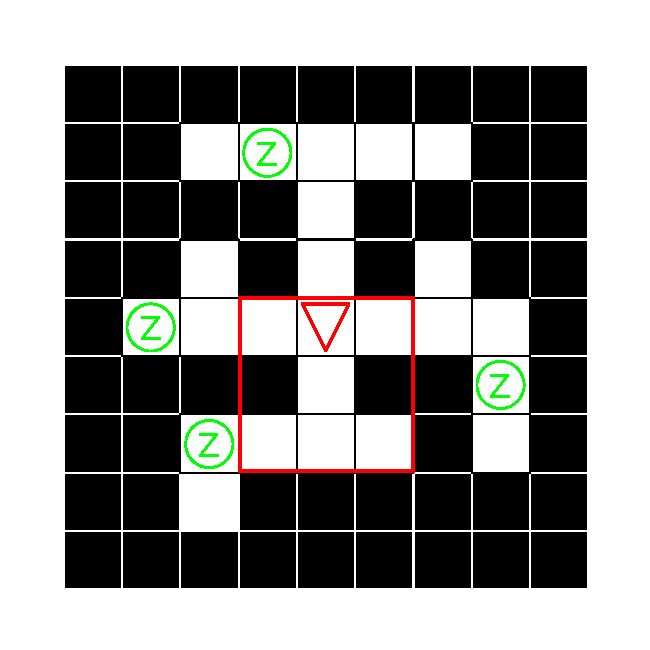
\includegraphics[keepaspectratio,width=0.5\textwidth]{abbildungen/fwmg.pdf}
  %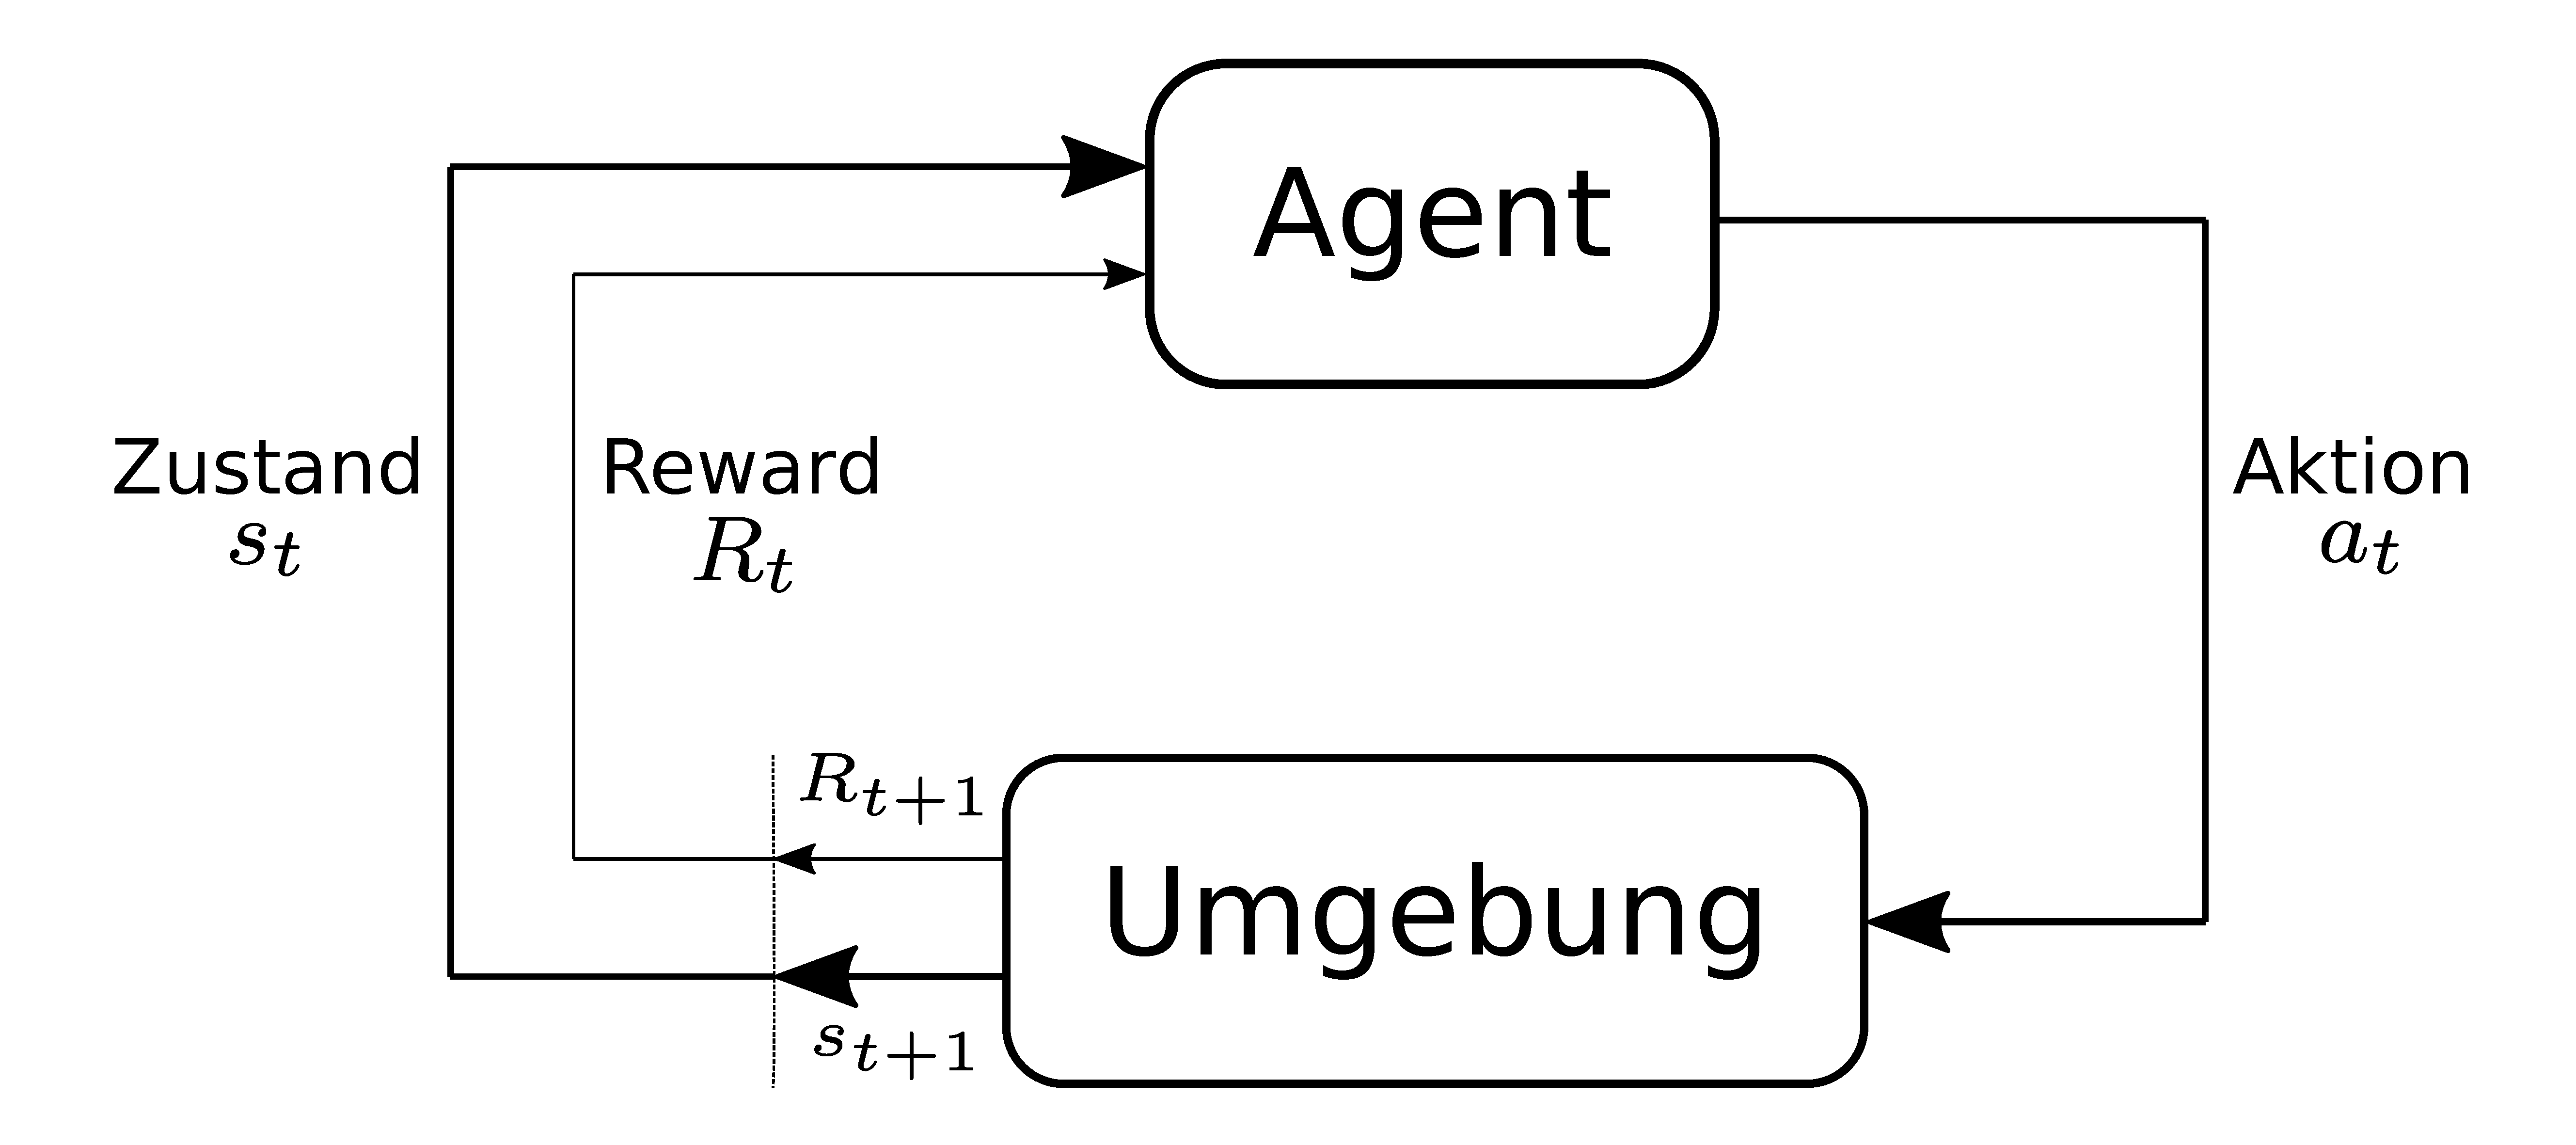
\includegraphics[height=0.5\textwidth, width=0.9\textwidth]{abbildungen/schnittstelle_agent_umgebung.pdf}
  \caption{Die Abbildung zeigt das Labyrinth der Umgebung \glqq Four\_Ways\_Many\_Goals\grqq{}. Der Agent startet zu Beginn jeder Episode auf dem zentralen Feld (rotes Dreieck) und erhält als Beobachtung einen Ausschnitt dem roten Rechteck entsprechend. Die grünen Kreise mit dem Buchstaben Z symbolisieren die möglichen Positionen zur Platzierung der Ziele.}
  \label{fig_fwmg_ep_start}
\end{figure}


Im Rahmen der folgenden Experimente soll ergründet werden, inwiefern die labyrinthartige Struktur der Umgebung einen Einfluss auf das Verhalten der verschiedenen Modelle hat. Dabei liegt wie in den vorherigen Experimenten der Fokus auf dem Erreichen von Zielen, die in der Vergangenheit bereits beobachtet wurden. Darüber hinaus ist von Interesse, ob die Gänge der Umgebung dazu führen, dass zukünftige Ziele öfter abgelaufen werden, anstatt beobachtet zu werden.

Die Umgebung \glqq Four\_Ways\_Many\_Goals\_2D \grqq{} ist eine 2D-Umgebung im Stile eines Labyrinths. Sie verfügt über eine fixe Größe von 9 Feldern in horizontaler Richtung und 9 Feldern in vertikaler Richtung. Vom zentralen Punkt der Umgebung geht in jede der vier Richtungen ein Weg aus. Dieser Weg verzweigt sich dann noch ein weiteres mal. Auf jedem Weg gibt es eine Position zur Platzierung eines Ziels. Zu Beginn einer Episode werden von diesen vier Position wahlweise zwei oder drei Ziele zufällig positioniert. Diese Ziele verfügen wieder über eine eindeutige Nummer. Der Agent beginnt jede Episode auf dem zentralen Feld in der Mitte und blickt dabei stets nach unten. Die Abbildung \ref{fig_fwmg_ep_start} zeigt das Labyrinth der Umgebung, die Startposition und -orientierung des Agenten (rotes Dreieck) und seine initiale Beobachtung (rotes Rechteck). Außerdem sind die möglichen Zielpositionen dargestellt in Form grüner Kreise mit dem Buchstaben Z. Die Aufgabe des Agenten besteht wieder darin, die Ziele in der korrekten Reihenfolge abzulaufen. Die dafür verwendete Struktur der Rewards sowie die maximale Schrittanzahl wird in Abhängigkeit der Anzahl der Ziele genauso gewählt wie in der Umgebung \glqq One\_Room\_Many\_Goals\grqq{} und kann somit der Tabelle \ref{belohnung_ormg} entnommen werden.

Dem Agenten stehen in jedem Schritt wieder die gleichen drei Aktionen zur Verfügung, d.h. gehe einen Schritt bzw. Feld nach vorne oder drehe dich um $90^\circ$ nach links oder rechts. Der Zustand $s_t$ ist hinsichtlich der binärkodierten Kanäle genauso aufgebaut wie bei der vorherigen Umgebung. Lediglich die Sichtreichweite in Blickrichtung wird um ein Feld reduziert. Somit ergibt sich die Größe des Zustands $s_t$ zu $(Anzahl\_Ziele + 1) \times 3 \times 3$.

Bei dieser Umgebung wird der Agent im Vergleich zur vorherigen Umgebung mit vorgegebenen Gängen bzw. Wegen konfrontiert. Somit ist seine Bewegungsmöglichkeit erheblich eingeschränkt. Darüber hinaus ist auch die Platzierung der Ziele restriktiver. Inwiefern diese Einschränkungen der Umgebung Auswirkungen auf das Verhalten der verschiedenen Neural Map Varianten und des LSTM hat, soll in den folgenden Experimenten geklärt werden.

Dabei werden wieder die zuvor beschriebenen vier Varianten der Neural Map und ein LSTM miteinander verglichen. Die Hyperparamter des PPO Algorithmus werden wie im vorherigen Abschnitt \ref{subsec_ormg} gewählt und können infolgedessen wieder in der Tabelle \ref{hyperparam_ppo_ormg} nachgeschaut werden. In Abhängigkeit der Anzahl der Ziele werden die Modelle zuerst wieder für eine entsprechende Schrittanzahl trainiert, ehe sie anschließend wieder für $10^5$ Schritte evaluiert werden.

\subsubsection{Zwei Ziele}

Zunächst werden in der in Abbildung \ref{fig_fwmg_ep_start} dargestellten Umgebung zufällig zwei Ziele platziert. Dazu werden zu Beginn jeder Episode von den vier möglichen Positionen zwei zufällig ausgewählt und mit den entsprechenden Zielen versehen. Alle Modelle werden für $2\cdot10^6$ Zeitschritte trainiert und anschließend wieder für $10^5$ Schritte evaluiert.

Die Auswertung folgt den vorherigen Experimenten. In Tabelle \ref{results_fwmg_2g} sind die Anzahl erfolgreicher Episoden, die durchschnittliche Schrittanzahl und der durchschnittliche Reward pro erfolgreicher Episode angegeben. Die Neural Map mit der Erweiterung des Schreiboperators (Neural Map + extW) erzielt die besten Ergebnisse, indem sie 2816 Episoden erfolgreich abschließt und dabei durchschnittlich 35,5 Schritte benötigt. Gefolgt wird sie von der Variante mit dem erweiterten Schreiboperator unter Verwendung der GRU-basierten Schreiboperation (Neural Map + extW + GRU), womit die beiden Varianten mit der Erweiterung des Schreiboperators bessere Ergebnisse erzielen als die Grundvarianten. In der Grundvariante verbessert die Verwendung der GRU-basierten Schreiboperation die Ergebnisse. Insgesamt liefern alle Varianten der Neural Map bessere Ergebnisse als das LSTM.

\begin{table}[ht!]
  \begin{tabular}{|>{\centering}m{5cm}|>{\centering}m{2.2cm}|>{\centering}m{3.5cm}|>{\centering}m{3.5cm}|} \hline
    Modell  & Anzahl erfolgreicher Episoden & Durchschnittliche Schrittanzahl pro erfolgreicher Episode & Durchschnittlicher Reward pro erfolgreicher Episode \tabularnewline \hline
    LSTM & 1978 & 49,3 & 0,54 \tabularnewline \hline
    Neural Map & 2253 & 41,7 & 0,64 \tabularnewline \hline
    Neural Map + GRU & 2136 & 40,0 & 0,66 \tabularnewline \hline
    Neural Map + extW & \textbf{2816} & \textbf{35,5} & \textbf{0,72} \tabularnewline \hline
    Neural Map + extW + GRU & 2619 & 36,7 & 0,71 \tabularnewline \hline
  \end{tabular}
  \caption{Übersicht über die Anzahl erfolgreicher Episoden, deren durchschnittliche Länge und durchschnittlicher Reward für die Umgebung \glqq Four\_Ways\_Many\_Goals\_2D\grqq{} mit zwei Zielen.}
  \label{results_fwmg_2g}
\end{table}

Als nächstes wird wieder der Weg von Ziel 1 zu Ziel 2 genauer betrachtet. Bei der Einteilung der Mengen ergibt sich, dass die Menge \glqq Ziel 2 nie beobachtet\grqq{} durchschnittlich 1249 Episoden enthält, die Menge \glqq Ziel 2 besucht\grqq{} 1194 Episoden und die Menge \glqq Ziel 2 gesehen\grqq{} 12 Episoden. Aufgrund der Tatsache, dass die zuletzt genannte Menge im Vergleich zu den beiden anderen nur über sehr wenige Episoden verfügt und für die Variante Neural Map + ExtW + GRU sogar komplett leer ist, werden die Mengen \glqq Ziel 2 besucht\grqq{} und \glqq Ziel 2 gesehen\grqq{} zusammengefasst zu der Menge \glqq Ziel 2 besucht / gesehen\grqq{}. Diese Menge enthält dann durchschnittlich 1206 Episoden. Die entsprechenden Ergebnisse befinden sich in der Tabelle \ref{results_fw2g_1_to_2_per_M}. Dabei fällt auf, dass alle Modelle in der Menge \glqq Ziel 2 nie beobachtet\grqq{} weniger zusätzliche Schritte benötigen. Die optimale Schrittanzahl ist für beide Menge sehr ähnlich und liegt zischen 7,7 und 8,0.

\begin{table}
  \begin{tabular}{|c|c|c|c|c|c|c|c|c|c|}
    \hline
    \multirow{3}{*}{Modell} & \multicolumn{3}{|c|}{Ziel 2 nie beobachtet} & \multicolumn{3}{|c|}{Ziel 2 besucht / gesehen} \\ \cline{2-7}
    & \multirow{2}{*}{Opt} & \multirow{2}{*}{Real} & rel. & \multirow{2}{*}{Opt} & \multirow{2}{*}{Real} & rel. \\
    & & & Diff & & & Diff \\ \hline
    LSTM & 7,6 & 23,1 & 204\% & 8,0 & 26,7 & 234\% \\ \hline
    Neural Map & 7,8 & 21,5 & 175\% & 7,8 & 23,0 & 193\% \\ \hline
    Neural Map + GRU & 7,8 & 20,1 & 157\% & 7,7 & 24,6 & 219\% \\ \hline
    Neural Map + extW & 7,8 & 17,0 & 118\% & 7,9 & 22,6 & 187\% \\ \hline
    Neural Map + extW + GRU & 7,9 & 19,3 & 146\% & 7,7 & 20,7 & 167\% \\ \hline
  \end{tabular}
  \caption{Übersicht über die optimale (Opt), tatsächliche (Real) und zusätzliche relative Schrittanzahl (rel. Diff) für den Weg von Ziel 1 zu Ziel 2 aufgeteilt in die zwei Mengen \glqq Ziel 2 nie beobachtet\grqq{} und \glqq Ziel 2 besucht / gesehen\grqq{} für die Umgebung \glqq Four\_Ways\_Many\_Goals\_2D\grqq{} mit zwei Zielen. Die Einteilung in die zwei Mengen erfolgt auf Basis der Observationen, die auf dem Weg zu Ziel 1 getätigt werden.}
  \label{results_fw2g_1_to_2_per_M}
\end{table}


\subsubsection{Drei Ziele}

Um die Schwierigkeit der Aufgabe zu erhöhen, werden im Folgenden drei Ziele in der Umgebung platziert, indem von den vier möglichen Positionen drei zufällig ausgewählt werden. Für das Training stehen in dieser Konfiguration $4\cdot10^5$ Schritte zur Verfügung, für die Evaluation $10^6$ Schritte. Die Gesamtergebnisse befinden sich in Tabelle \ref{results_fwmg_3g}. Mit 1926 erfolgreich absolvierten Episoden erreicht die Neural Map mit der Erweiterung des Schreiboperators unter Verwendendung der GRU-basierten Schreiboperation die besten Ergebnisse. Sie benötigt durchschnittlich 51,7 Schritte für eine erfolgreiche Episode. Gefolgt wird sie von der Variante mit dem erweiterten Schreiboperator, womit beide Varianten mit selbigem besser abschneiden als die Grundvarianten der Neural Map. Außerden verbessert die GRU-basierte Schreiboperation beide Varianten. Insgesamt erzielen alle Varianten der Neural Map bessere Ergebnisse als das LSTM.

\begin{table}[ht!]
  \begin{tabular}{|>{\centering}m{5cm}|>{\centering}m{2.2cm}|>{\centering}m{3.5cm}|>{\centering}m{3.5cm}|} \hline
    Modell  & Anzahl erfolgreicher Episoden & Durchschnittliche Schrittanzahl pro erfolgreicher Episode & Durchschnittlicher Reward pro erfolgreicher Episode \tabularnewline \hline
    LSTM & 1349 & 74,1 & 1,03 \tabularnewline \hline
    Neural Map & 1579 & 63,3 & 1,08 \tabularnewline \hline
    Neural Map + GRU & 1659 & 60,3 & 1,09 \tabularnewline \hline
    Neural Map + extW & 1783 & 57,7 & 1,11 \tabularnewline \hline
    Neural Map + extW + GRU & \textbf{1926} & \textbf{51,7} & \textbf{1,14} \tabularnewline \hline
  \end{tabular}
  \caption{Übersicht über die Anzahl erfolgreicher Episoden, deren durchschnittliche Länge und durchschnittlicher Reward für die Umgebung \glqq Four\_Ways\_Many\_Goals\_2D\grqq{} mit drei Zielen.}
  \label{results_fwmg_3g}
\end{table}

Als nächstes wird wieder der Weg von Ziel 1 zu Ziel 2 genauer untersucht. Die Mengen \glqq Ziel 2 besucht\grqq{} und \glqq Ziel 2 gesehen\grqq{} werden aus den gleichen Gründen wie im vorherigen Experiment zur Menge \glqq Ziel 2 besucht / gesehen\grqq{} zusammengefasst. Diese enthält durchschnittlich 846 Episoden und die Menge \glqq Ziel 2 nie beobachtet\grqq{} 760 Episoden. In der Tabelle \ref{results_fw3g_1_to_2_per_M} sind die Ergebnisse zusammengefasst. Es ist wieder auffallend, dass alle Modelle in der Menge \glqq Ziel 2 nie beobachtet\grqq{} weniger zusätzliche Schritte benötigen. Darüber hinaus ist die optimale Schrittanzahl in dieser Menge ungefähr um einen halben Schritt größer, ausgenommen die Variante Neural Map + extW + GRU.

\begin{table}[h]
  \begin{tabular}{|c|c|c|c|c|c|c|c|c|c|}
    \hline
    \multirow{3}{*}{Modell} & \multicolumn{3}{|c|}{Ziel 2 nie beobachtet} & \multicolumn{3}{|c|}{Ziel 2 besucht / gesehen} \\ \cline{2-7}
    & \multirow{2}{*}{Opt} & \multirow{2}{*}{Real} & rel. & \multirow{2}{*}{Opt} & \multirow{2}{*}{Real} & rel. \\
    & & & Diff & & & Diff \\ \hline
    LSTM & 7,8 & 20,7 & 165\% & 7,3 & 26,9 & 269\% \\ \hline
    Neural Map & 7,7 & 18,4 & 138\% & 7,2 & 26,3 & 263\% \\ \hline
    Neural Map + GRU & 7,8 & 17,9 & 129\% & 7,1 & 23,0 & 224\% \\ \hline
    Neural Map + extW & 7,7 & 19,5 & 151\% & 7,2 & 25,7 & 255\% \\ \hline
    Neural Map + extW + GRU & 7,5 & 17,6 & 135\% & 7,5 & 21,5 & 188\% \\ \hline
  \end{tabular}
  \caption{Übersicht über die optimale (Opt), tatsächliche (Real) und zusätzliche relative Schrittanzahl (rel. Diff) für den Weg von Ziel 1 zu Ziel 2 aufgeteilt in die zwei Mengen \glqq Ziel 2 nie beobachtet\grqq{} und \glqq Ziel 2 besucht / gesehen\grqq{} für die Umgebung \glqq Four\_Ways\_Many\_Goals\_2D\grqq{} mit drei Zielen. Die Einteilung in die zwei Mengen erfolgt auf Basis der Observationen, die auf dem Weg zu Ziel 1 getätigt werden.}
  \label{results_fw3g_1_to_2_per_M}
\end{table}

Der Weg von Ziel 2 zu Ziel 3 wird erneut detaillierter analysiert, wozu wieder die zwei Mengen \glqq Ziel 3 nie beobachtet\grqq{} und \glqq Ziel 3 besucht / gesehen\grqq{} gebildet. Erstere enthält durchschnittlich 237 Episoden und Zweitere 1369 Episoden. Die resultierenden Ergebnisse befinden sich in der Tabelle \ref{results_fw3g_2_to_3_per_M}. Wieder benötigen alle Modelle in der Menge \glqq Ziel 3 nie beobachtet\grqq{} weniger zusätzliche Schritte. Darüber hinaus ist der optimale Weg in dieser Menge im Durchschnitt über alle Modelle wieder ungefähr um einen halben Schritt größer.

\begin{table}[h]
  \begin{tabular}{|c|c|c|c|c|c|c|c|c|c|}
    \hline
    \multirow{3}{*}{Modell} & \multicolumn{3}{|c|}{Ziel 3 nie beobachtet} & \multicolumn{3}{|c|}{Ziel 3 besucht / gesehen} \\ \cline{2-7}
    & \multirow{2}{*}{Opt} & \multirow{2}{*}{Real} & rel. & \multirow{2}{*}{Opt} & \multirow{2}{*}{Real} & rel. \\
    & & & Diff & & & Diff \\ \hline
    LSTM & 8,0 & 16,7 & 107\% & 7,7 & 27,0 & 249\% \\ \hline
    Neural Map & 8,9 & 14,3 & 61\% & 7,7 & 24,3 & 215\% \\ \hline
    Neural Map + GRU & 8,1 & 15,1 & 86\% & 7,7 & 22,8 & 195\% \\ \hline
    Neural Map + extW & 7,7 & 17,0 & 119\% & 7,8 & 23,5 & 202\% \\ \hline
    Neural Map + extW + GRU & 8,8 & 13,5 & 52\% & 7,7 & 16,2 & 111\% \\ \hline
  \end{tabular}
  \caption{Übersicht über die optimale (Opt), tatsächliche (Real) und zusätzliche relative Schrittanzahl (rel. Diff) für den Weg von Ziel 2 zu Ziel 3 aufgeteilt in die zwei Mengen \glqq Ziel 3 nie beobachtet\grqq{} und \glqq Ziel 3 besucht / gesehen\grqq{} für die Umgebung \glqq Four\_Ways\_Many\_Goals\_2D\grqq{} mit drei Zielen. Die Einteilung in die zwei Mengen erfolgt auf Basis der Observationen, die auf dem Weg zu Ziel 2 getätigt werden.}
  \label{results_fw3g_2_to_3_per_M}
\end{table}


\section{3D-Experiment}
\label{sec_3d_exp}

Nachdem zuvor das Verhalten der Neural Map in verschiedenen 2D-Umgebungen ausführlich untersucht wurde, soll nun eine 3D-Umgebung verwendet werden. Hierbei soll geklärt werden, inwiefern die Ergebnisse aus den 2D-Umgebungen auch in einer 3D-Umgebung Bestand haben.

Die 3D-Umgebung wird auf Basis von ViZDoom erstellt \cite{VizDoom}. ViZDoom basiert auf dem Computerspiel Doom und ermöglicht es, selbiges im RL Kontext zu benutzen. Somit lassen sich die Tastendrücke als Aktionen ausführen. Es kann auf den Bildschirminhalt zugegriffen werden, sodass dieser als Observation verwendet werden kann. Außerdem lassen sich auf Basis einer spieleigenen Scriptsprache gewisse Events mit entsprechenden Rewards verknüpfen. Darüber hinaus sind ein Schrittlimit sowie ein Living-Reward bereits implementiert und müssen nur mit entsprechenden Werten ausgestattet werden.

Die Umgebung ist eine Adaption der 2D-Umgebung \glqq One\_Room\_Many\_Goals\grqq{}. Sie besteht somit aus einem quadratischem Raum. In diesem Raum werden zufällig zwei Ziele platziert, eine grüne Säule und eine rote Säule. Für die Platzierung der Ziele stehen insgesamt 20 mögliche Positionen zur Verfügung, wobei diese auf die beiden Raumhälften aufgeteilt sind. Zunächst wird zufällig eine dieser Positionen für das grüne Ziel ausgewählt. Um zu verhindern, dass die beiden Ziele zu nah beieinander liegen, stehen für die anschließende Platzierung des roten Ziels nur die Positionen in der anderen Raumhälfte zur Verfügung (also 10). Der Agent startet immer auf einer fixen Position in der Mitte des Raumes, die initiale Blickrichtung ist ebenfalls immer dieselbe. Die Aufgabe des Agenten ist es, zuerst zur grünen Säule und dann zur roten Säule zu laufen. Hierfür erhält er für das Erreichen der grünen Säule einen Reward von 0,2 und für das Erreichen der roten Säule einen Reward von 1,0. Das jeweilige Ziel gilt als erreicht, sobald der Agent sich ihm bis auf eine gewisse Entfernung genähert hat. Dazu wird über den Mittelpunkt der Säulen jeweils ein Kreis gelegt. Zum Bewältigen dieser Aufgabe stehen dem Agenten 5000 Schritte zur Verfügung. Für jeden Schritt erhält er einen Living-Reward von $-0,0002$. Der Agent kann zwischen den drei Aktionen \glqq Drehung links\grqq{}, \glqqDrehung rechts\grqq{} und \glqq Gehe geradeaus\grqq{} auswählen. Dazu erhält er als Observation ein RGB-Array der Dimensionalität $120 \times 160 \times 3$.

Da die $x$- und $y$-Koordinate des Agenten Werte zischen 0 und 800 einnehmen kann, wird die in Abschnitt \ref{sec_neural_map} erwähnte Koordinatennormalisierungsfunktion $\psi$ in diesem Experiment benötigt. Der interne Speicher der Neural Map hat in horizontaler und vertikaler Richtung wieder jeweils die Größe 15. Um die Position des Agenten in der Umgebung auf eine gültige Speicherposition abzubilden, wird $\psi(x) = \lfloor x / 534\rfloor$ gewählt. Die Gaußklammern sind als ganzzahlige Division implementiert, sodass das Ergebnis abgerundet bzw. abgeschnitten wird. Darüber hinaus benutzen alle Varianten der Neural Map die in Abschnitt \ref{sec_nm_3d_ext} erwähnte Erweiterung für 3D-Umgebungen. Das LSTM nutzt diese ebenfalls zur Vorverarbeitung der Observation, d.h. die Observation wird zunächst von dem entsprechenden Neuronalen Faltungsnetz verarbeitet und dessen Ausgabe bildet dann die Eingabe des LSTM.

Die für das Training verwendeten Hyperparameter des PPO Algorithmus können der Tabelle \ref{hyperparam_ppo_3d} entnommen werden. Alle Modelle werden für $10\cdot10^6$ Zeitschritte trainiert und anschließend für $10^6$ Schritte evaluiert. Im Rahmen dieser Evaluation werden wieder für jede Episode der Reward und die Länge aufgezeichnet.

\begin{table}[h]
  \begin{center}
    \begin{tabular}{1 1}
      \hline
      nsteps & $2048$ \\
      ent\_coef & $0.01$ \\
      lr & $3\cdot10^{-4}$ \\
      vf\_coef & $0,5$ \\
      max\_grad\_norm & $0,5$ \\
      gamma & $0,99$ \\
      noptepochs & $4$ \\
      cliprange & $0,2$ \\
      \hline
    \end{tabular}
  \end{center}
  \caption{Übersicht über die zum Training in der 3D-Umgebung verwendeten Hyperparameter des PPO Algorithmus.}
  \label{hyperparam_ppo_3d}
\end{table}

Die Durchschnittswerte des Rewards und der Episodenlänge über die erfolgreichen Episoden sowie die Anzahl erfolgreicher Episoden können der Tabelle \ref{results_3d} entnommen werden. Hierbei erzielt die Neural Map mit der Erweiterung des Schreiboperators unter Verwendung der GRU-basierten Schreiboperation die besten Resultate. Sie absolvierte 516 erfolgreiche Episoden und benötigte dafür durchschnittlich 1768,5 Schritte. Gefolgt wird sie von der Variante Neural Map + extW, womit die Varianten mit der Erweiterung des Schreiboperators bessere Ergebnisse erzielen als die Grundvarianten. Danach folgt die Grundvariante, die die GRU-basierte Schreiboperation verwendet. Demnach verbessert die Benutzung der GRU-basierten Schreiboperation die jeweilige Variante der Neural Map. Darüber hinaus erreichen alle Varianten der Neural Map bessere Ergebnisse als das LSTM.

\begin{table}[ht!]
  \begin{tabular}{|>{\centering}m{5cm}|>{\centering}m{2.2cm}|>{\centering}m{3.5cm}|>{\centering}m{3.5cm}|} \hline
    Modell  & Anzahl erfolgreicher Episoden & Durchschnittliche Schrittanzahl pro erfolgreicher Episode & Durchschnittlicher Reward pro erfolgreicher Episode \tabularnewline \hline
    LSTM & 451 & 1943,8 & 0,81 \tabularnewline \hline
    Neural Map & 474 & 1866,2 & 0,83 \tabularnewline \hline
    Neural Map + GRU & 483 & 1839,7 & 0,83 \tabularnewline \hline
    Neural Map + extW & 499 & 1805,0 & 0,84 \tabularnewline \hline
    Neural Map + extW + GRU & \textbf{516} & \textbf{1768,5} & \textbf{0,85} \tabularnewline \hline
  \end{tabular}
  \caption{Übersicht über die Anzahl erfolgreicher Episoden, deren durchschnittliche Länge und durchschnittlicher Reward für die 3D-Umgebung.}
  \label{results_3d}
\end{table}

\section{Untersuchung der Neural Map als reine Speicherstruktur}
\label{sec_mem_test}

Im abschließenden Experiment soll die Neural Map außerhalb des bisherigen RL Kontexts untersucht werden. Es soll herausgefunden werden, inwiefern sich die Neural Map als reine Speicherstruktur nutzen lässt. Hierbei ist insbesondere von Interesse, inwiefern die Neural Map in ihrem internen Speicher eine Karte der Umgebung generieren kann. Um dies zu ergründen, wird eine leicht abgeänderte Form der Neural Map im Supervised Lernkontext betrachtet. Dazu werden folgende Annahmen getätigt. Zunächst wird wie in den 2D-Experimenten die vertikale und horizontale Größe des internen Speichers entsprechend der Umgebungsgröße gewählt. Somit entspricht eine Position in der Umgebung exakt einer Speicherposition. Die Informationen über die Umgebung, d.h. das Vorhandensein von Wänden bzw. freien Feldern und die Lage der Ziele, sind wie in den Abschnitten \ref{subsec_ormg} und \ref{subsec_fwmg} beschrieben binär kodiert. Daraus ergibt sich, dass für jede Position der Umgebung ein entsprechend binärkodierter Umgebungsvektor existiert. Da es zu jeder Position in der Umgebung genau eine Position im internen Speicher gibt und sich das Feature an dieser Speicherposition nur durch seine Dimensionalität von dem Umgebungsvektor unterscheidet, wird das Feature als kodierte Form des Umgebungsvektors angesehen. Dabei ist die Kodierung zunächst unbekannt. Auf Basis dieser Annahmen wird für das Experiment eine leicht modifizierte Variante der Neural Map erstellt. Diese erhält als Eingabe wie gehabt eine Observation $s_t$ und den aktuellen Inhalt des internen Speichers $M_t$ und schätzt auf Basis dieser den Umgebungsvektor an der entsprechenden Position $(x_t, y_t)$. Im Fall der Neural Map mit der Erweiterung des Schreibvektors wird zusätzlich auch noch der Umgebungsvektor an der Position $(x_{ext_t},y_{ext_t})$ geschätzt. Im Folgenden wird zugunsten einer besseren Lesbarkeit darauf verzichtet, wiederholt darauf hinzuweisen, dass in Abhängigkeit der Benutzung des erweiterten Schreiboperators wahlweise ein oder zwei Vektoren von der modifizierten Variante der Neural Map geschätzt bzw. erzeugt werden.

Die für die Experimente benötigten Daten bilden Paare der Form (Eingabe, wahre Ausgabe). Um diese zu generieren, werden die 2D-Umgebungen um eine zusätzliche Methode ergänzt. Diese erzeugt eine zufällige Observation aus der entsprechenden Umgebung. Dazu wird zunächst zufällig eine gültige Position des Agenten bestimmt, d.h. eine Position auf einem freien Feld. Anschließend wird auch die Orientierung zufällig gewählt und die zu der Positon und Orientierung gehörige Observation zurückgegeben. Da im Supervised Kontext auch die wahre Ausgabe bekannt sein muss, wird eine weitere Methode benötigt. Diese gibt die gesamte Umgebung zurück, d.h. die Umgebungsvektoren für alle Positionen, und wird einmal zu Beginn des Experiments aufgerufen. Im weiteren Verlauf können dann hieraus die jeweils benötigten Umgebungsvektoren auf Basis der Positionen extrahiert werden. Auf diese Weise werden die benötigten paarweisen Datenpunkte generiert.

Da die Neural Map nun als Ausgabe auch einen Vektor mit der gleichen Dimensionalität wie der des Umgebungsvektors erzeugen muss, wird sie entsprechend modifiziert. Dazu wird zunächst das finale Neuronale Netz der Neural Map entfernt, da dessen Zweck in der Schätzung der Policy liegt und diese in diesem Experiment nicht benötigt wird. Das so veränderte Modell erzeugt als Ausgabe den Schreibvektor $w_{t+1}^{(x_t,y_t)}$ mittels der Local Write Operation. Da dieser noch über eine andere Dimensionalität als der Umgebungsvektor verfügt, wird er anschließend von einer weiteren Fully-Connected Schicht verarbeitet. Diese kann als Dekoder angesehen werden, da sie zur Schätzung des Umgebungsvektors das entsprechend kodierte Feature dekodiert. Somit generiert die entsprechend abgeänderte Neural Map als Ausgabe einen Vektor in der gleichen Dimensionalität wie der Umgebungsvektor. Damit die Einträge des geschätzten Umgebungsvektors auch aus dem Intervall $[0, 1]$ kommen, wird als Aktivierungsfunktion in der Dekoder-Schicht die Sigmoid-Funktion für beide Modelle verwendet.

Nun kann wie im Supervised Kontext üblich die Ausgabe des Modells, also die Schätzung, mit der wahren Ausgabe verglichen werden, indem die Differenz der beiden Vektoren gebildet wird. Auf diesen Differenzvektor wird dann der Mean-Squared-Error als Fehlermaß angewendet. Die so entstehende Verlustfunktion kann nun mit einem entsprechenden Optimierer minimiert werden. Dazu berechnet selbiger den Gradienten des Modells und ändert auf Basis dessen die Parameter des Modells. Hierzu wird der sogenannte Adam Optimierer verwendet \cite{Adam}. Seine Parameter entsprechen den Standardwerten und als Lernrate wird $3\ctimes10^{-4}$ verwendet. Die Modelle werden jeweils für $25.000$ Schritte trainiert.

Für die Experimente wird zum einen die Umgebung \glqq One\_Room\_Many\_Goals\grqq{} in der Größe $9 \times 9$ mit vier Zielen verwendet und die Umgebung \glqq Four\_Ways\_Many\_Goals\grqq{} ebenfalls mit vier Zielen. Als Modelle werden die Grundvariante der Neural Map und die Variante mit der Erweiterung des Schreiboperators betrachtet. Von jeder der beiden Umgebungen werden zehn zufällige Konfigurationen verwendet, auf Basis derer die beiden Modelle trainiert werden. Eine Konfiguration entspricht dabei einer bestimmten Platzierung der vier Ziele und wird paarweise für beide Modelle verwendet, um die entsprechenden Ergebnisse vergleichen zu können. Lediglich die zum Training verwendeten zufälligen Observationen unterscheiden sich noch. Da die Grundvariante der Neural Map nur gültige bzw. freie Felder beschreiben kann, werden auch nur diese bei dem abschließenden Vergleich der beiden Modelle betrachtet. Hierzu wird nach Ende des Traingsprozesses die Güte der erzeugten Karte bewertet, indem für alle zuvor erwähnten Positionen die Differenz zwischen den geschätzten und tatsächlichen Umgebungsvektoren bestimmt wird und auf diesen anschließend der Mean-Squared-Error berechnet wird. In einem weiteren Bewertungsansatz werden die Einträge der geschätzten Umgebungsvektoren mittels eines Schwellwertes von 0,2 bzw. 0,8 wahlweise zu Null oder Eins gesetzt. Anschließend werden die Vektoren entsprechend ihrer Positionen wieder zu einer Karte zusammengesetzt und es wird überprüft, ob die tatsächlichen Positionen der Ziele aus der geschätzten Karte korrekt rekonstruiert werden können.

Die Abbildungen \ref{fig_mem_test_ormg} und \ref{fig_mem_test_fwmg} zeigen beispielhafte Verläufe des Mean-Squared-Errors über die Anzahl der Trainingschritte für die jeweiligen Umgebungen. Dabei ist auffällig, dass der MSE zu Beginn des Trainings relativ schnell bis auf ungefähr $0,2$ abfällt, wo er dann für eine längere Zeit verweilt, bevor er wiederum weiter abfällt und seinen Endwert erreicht. In allen betrachteten Konfigurationen liegt der MSE für beide Modelle am Ende des Trainings in der Größenordnung zwischen $10^{-4}$ und $10^{-5}$. Diese Werte werden auch für beide Modelle bei der zuvor beschriebenen abschließenden Güteberechnung der Karte erreicht. Bei der Anwendung des zuvor erwähnten Schwellwertansatzes können in allen Experimenten die Positionen der Ziele fehlerfrei rekonstruiert werden. Abschließend lässt sich festhalten, dass beide betrachten Modelle, sprich die Neural Map mit und ohne Erweiterung des Schreiboperators, in der Lage sind, entsprechende Karten der jeweiligen Umgebungen zu generieren. Ein Unterschied in der Qualität der erzeugten Karten und in der dazu benötigten Anzahl von Zeit- bzw. Trainingsschritten konnte anhand der verwendeten Bewertungskriterien nicht ausgemacht werden.


\begin{figure}[ht!]
  \centering
  %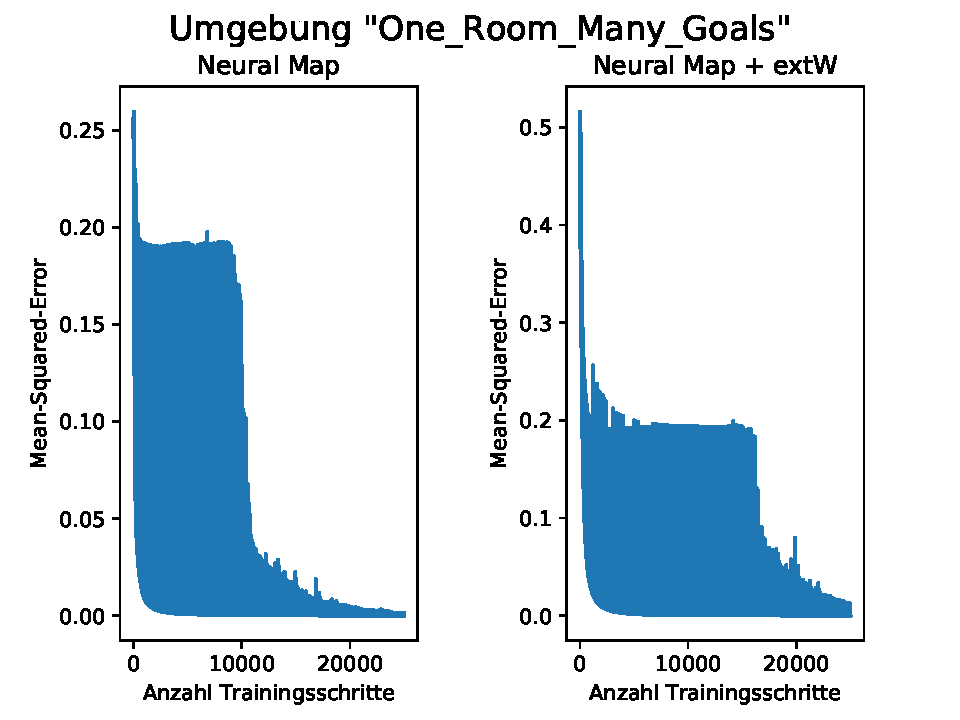
\includegraphics[keepaspectratio,width=1.0\textwidth]{abbildungen/mem_test_ormg.pdf}
  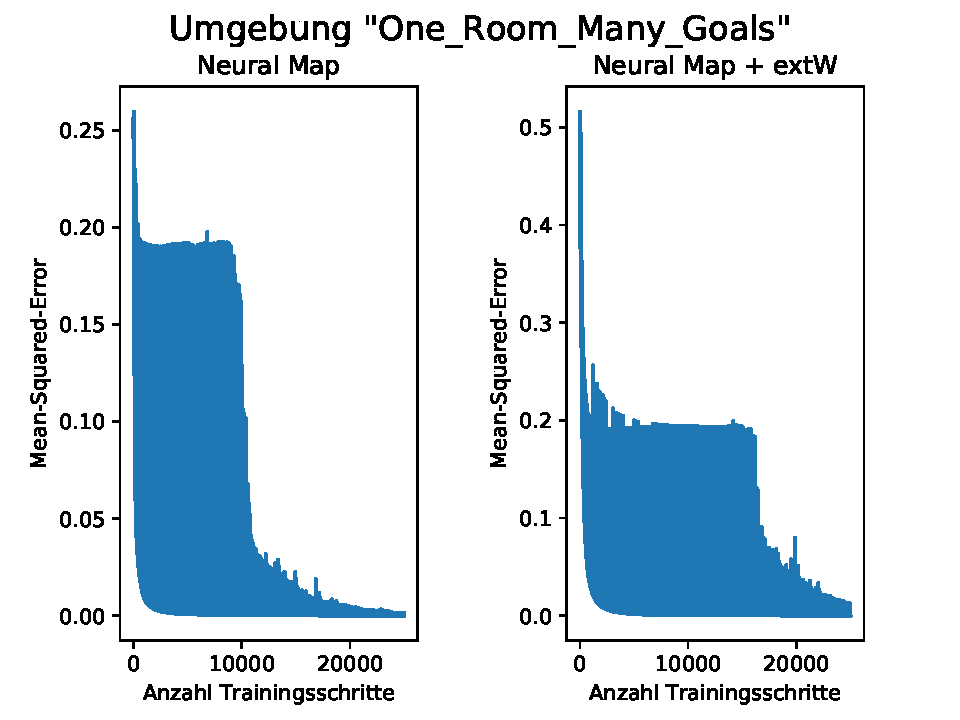
\includegraphics[height=0.575\textwidth, width=0.9\textwidth]{abbildungen/mem_test_ormg.pdf}
  \caption{Die Abbildung zeigt die Entwicklung des Mean-Squared-Error über die Anzahl der Trainingschritte für die Neural Map und die Neural Map mit der Erweiterung des Schreiboperators für die Umgebung \glqq One\_Room\_Many\_Goals\grqq{}.}
  \label{fig_mem_test_ormg}
\end{figure}

\begin{figure}[ht!]
  \centering
  %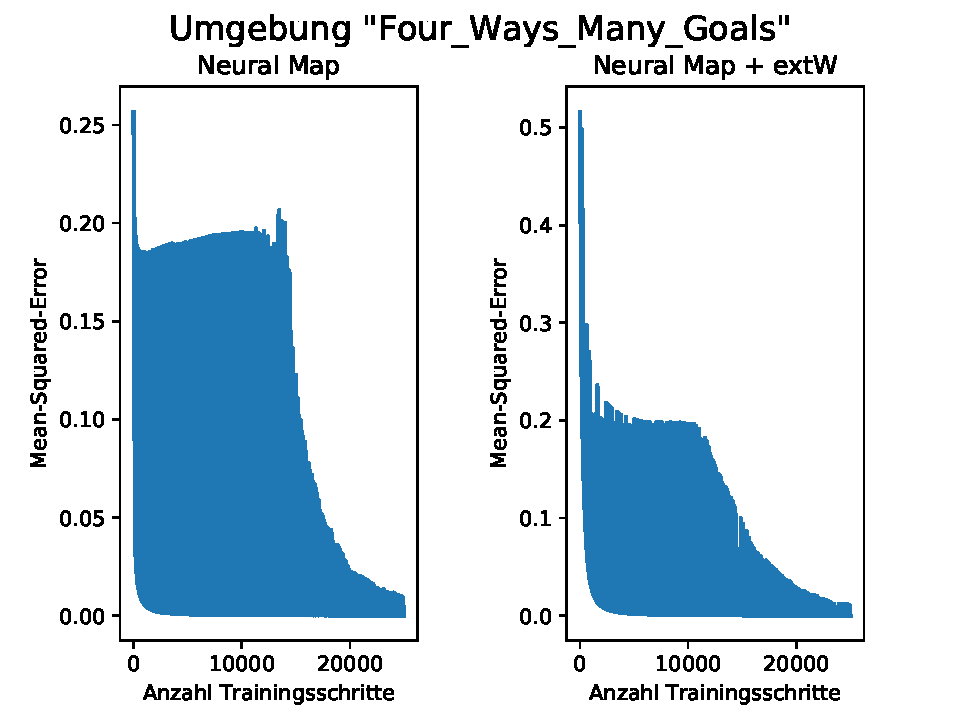
\includegraphics[keepaspectratio,width=1.0\textwidth]{abbildungen/mem_test_fwmg.pdf}
  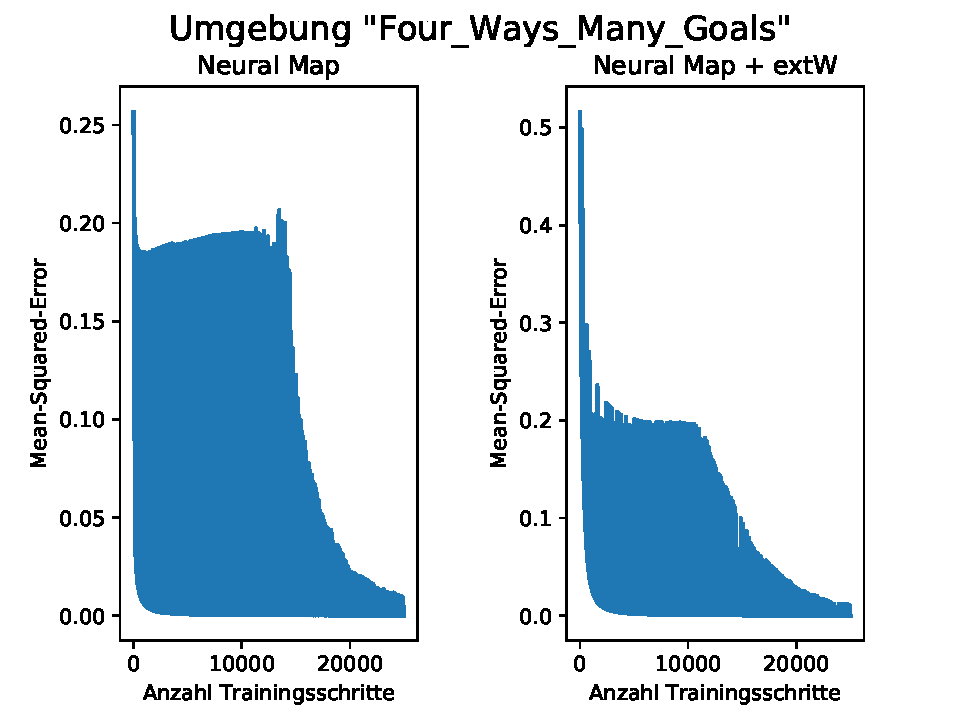
\includegraphics[height=0.575\textwidth, width=0.9\textwidth]{abbildungen/mem_test_fwmg.pdf}
  \caption{Die Abbildung zeigt die Entwicklung des Mean-Squared-Error über die Anzahl der Trainingschritte für die Neural Map und die Neural Map mit der Erweiterung des Schreiboperators für die Umgebung \glqq Four\_Ways\_Many\_Goals\grqq{}.}
  \label{fig_mem_test_fwmg}
\end{figure}
